\documentclass[preview,12pt]{article}
\usepackage{amsmath}
\usepackage{gensymb}
\usepackage{ragged2e}
\usepackage{geometry}
\usepackage{graphicx}
\usepackage{caption}
\usepackage{subcaption}
\usepackage{pdfpages}

\geometry{letterpaper, margin=1in}

\begin{document}

\begin{titlepage}
    \vspace*{\fill}
    \begin{center}
        \LARGE \textit{"Measurement of Turbulent Concentration Field of Acetone-Seeded Air Jet using Planar Laser Induced Fluorescence"}
    \end{center}
    \begin{center}
       \large Josh Coffey
    \end{center}
    \begin{center}
        \large University of Cincinnati
    \end{center}
    \begin{center}
        \large December 2019
    \end{center}
        \vspace*{\fill}
\end{titlepage}

\begin{center}
    \section*{Introduction}
\end{center}
\subsection*{Principle of Laser Induced Fluorescence Measurement of Concentration}
\indent Laser induced fluorescence (LIF) is "the spontaneous emission of radiation resulting from the stimulation of an atomic or molecular system by a laser" to a higher energy state [1].  In other words, the laser beam will excite an atom or molecule to a higher energy state through absorption and when the atom or molecule returns to a lower energy state, it will emit a photon.  The laser is chosen so that it is resonant with the desired energy transition, which is determined using the equation:
$$E=\frac{hc}{\lambda}$$
where $\lambda$ is the wavelength associated with the change in energy state.
It is a method of measuring the concentration of a species in an airflow.  Unlike other methods of measurement, such as absorption, LIF is not line of sight and gives a point measurement, rather than an average measurement over the laser's path.  In addition, it has the advantage of being non-intrusive, so the measurement does not change the flow field, and real-time, so the measurement taken reflects what is happening at the moment. One of the main disadvantages of LIF is that it is very sensitive to light, including light that is in the background and is not part of the laser.  This can include light from LIF of other species, scattered light from the surroundings, particle incandescence, and gas breakdown. \newline
\indent In LIF, a laser is directed through an air jet.  A detector is set up so that measurements can be taken in the air jet at the point at which the light that reaches the detector intersects with the laser beam passing through the jet. In other words, the fluorescence is measured at 90\degree  from the laser beam.  The measured fluorescence is related to the population of the excited state: the more fluorescence is measured, the higher the population of the excited state.  At thermodynamic equilibrium, the population of the excited state is proportional to the population of the ground state, which gives a value for the population of the desired species.

\subsection*{Measurement Principle for Acetone LIF}
Because the measured fluorescence is proportional to the population of the ground state at thermodynamic equilibrium, the intensity of the fluorescence can be used to find the concentration of the wanted species.  In other words, the concentration of acetone, or whichever tracer is used, is related to the intensity of the laser induced fluorescence of the jet. 
\newline
\indent Quenching is when the there are collisions between the photons and molecules in the medium that the laser is passing through.  Specifically, molecules other than the ones that the laser is meant to increase the energy level of.  This causes an energy loss from the photons which causes radiative decay from the excited state and interferes with the output signal.  Quenching must be taken into account when calculating the total fluorescence.  Because the concentration of a species is found because of how much that species fluoresces, anything that reduces  or changes that fluorescence will lead to an incorrect concentration calculation.  It is also possible for the opposite to happen: because of a factor outside of the experiment, the fluorescence can increase, thus leading to a higher concentration than is accurate.  \newline
\indent One factor that can affect fluorescence is pressure.  Studies have shown that as pressure increases, so to does the fluorescence, although the effect is reduced as pressure gets higher [2].  In addition, other studies have shown that as pressure increases, quantum efficiency, or the efficiency at which photons are released, increases [3].\newline
\indent Another factor that affects fluorescence is the composition of the gas. The same study that found that the quantum efficiency changes with pressure found that the species that comprises the buffer gas can also change the quantum efficiency [3].  They found that when the buffer gas is air, the quantum efficiency of the acetone decreases, while for nitrogen, methane, and helium the quantum efficiency is not affected.  Another study found that oxygen as the buffer gas increases quenching [5].  Another way that composition changes the fluorescence is in the tracer itself.  While acetone is the most commonly used tracer, it is not the only possibility and each tracer will have different properties [2].  This will have a large impact, on everything from the amount of quenching that occurs to the wavelength of the produced photon. \newline
\indent Temperature can also impact the resulting fluorescence.  One study found that as temperature increases, so to does the wavelength of acetone emissions, and that as temperature increases, the fluorescence of several wavelengths tended to decrease [4].
\newline
\indent Planar LIF is when the laser beam is spread using a lens into a flat sheet.  This flat column of laser is then sent through the jet and a camera at 90\degree to the plane is able to take images of the resulting fluorescence.  In PLIF, a camera replaces the photomultiplier tube that is used to detect the signal in LIF.  The camera must be equipped with a bandpass filter to allow in only the desired frequencies. The advantage of PLIF is that it allows direct imaging of the jet at a certain point. 
\newpage

\begin{center}
    \section*{Experimental Setup and Procedure}
\end{center}

\begin{figure}[h]
    \centering
    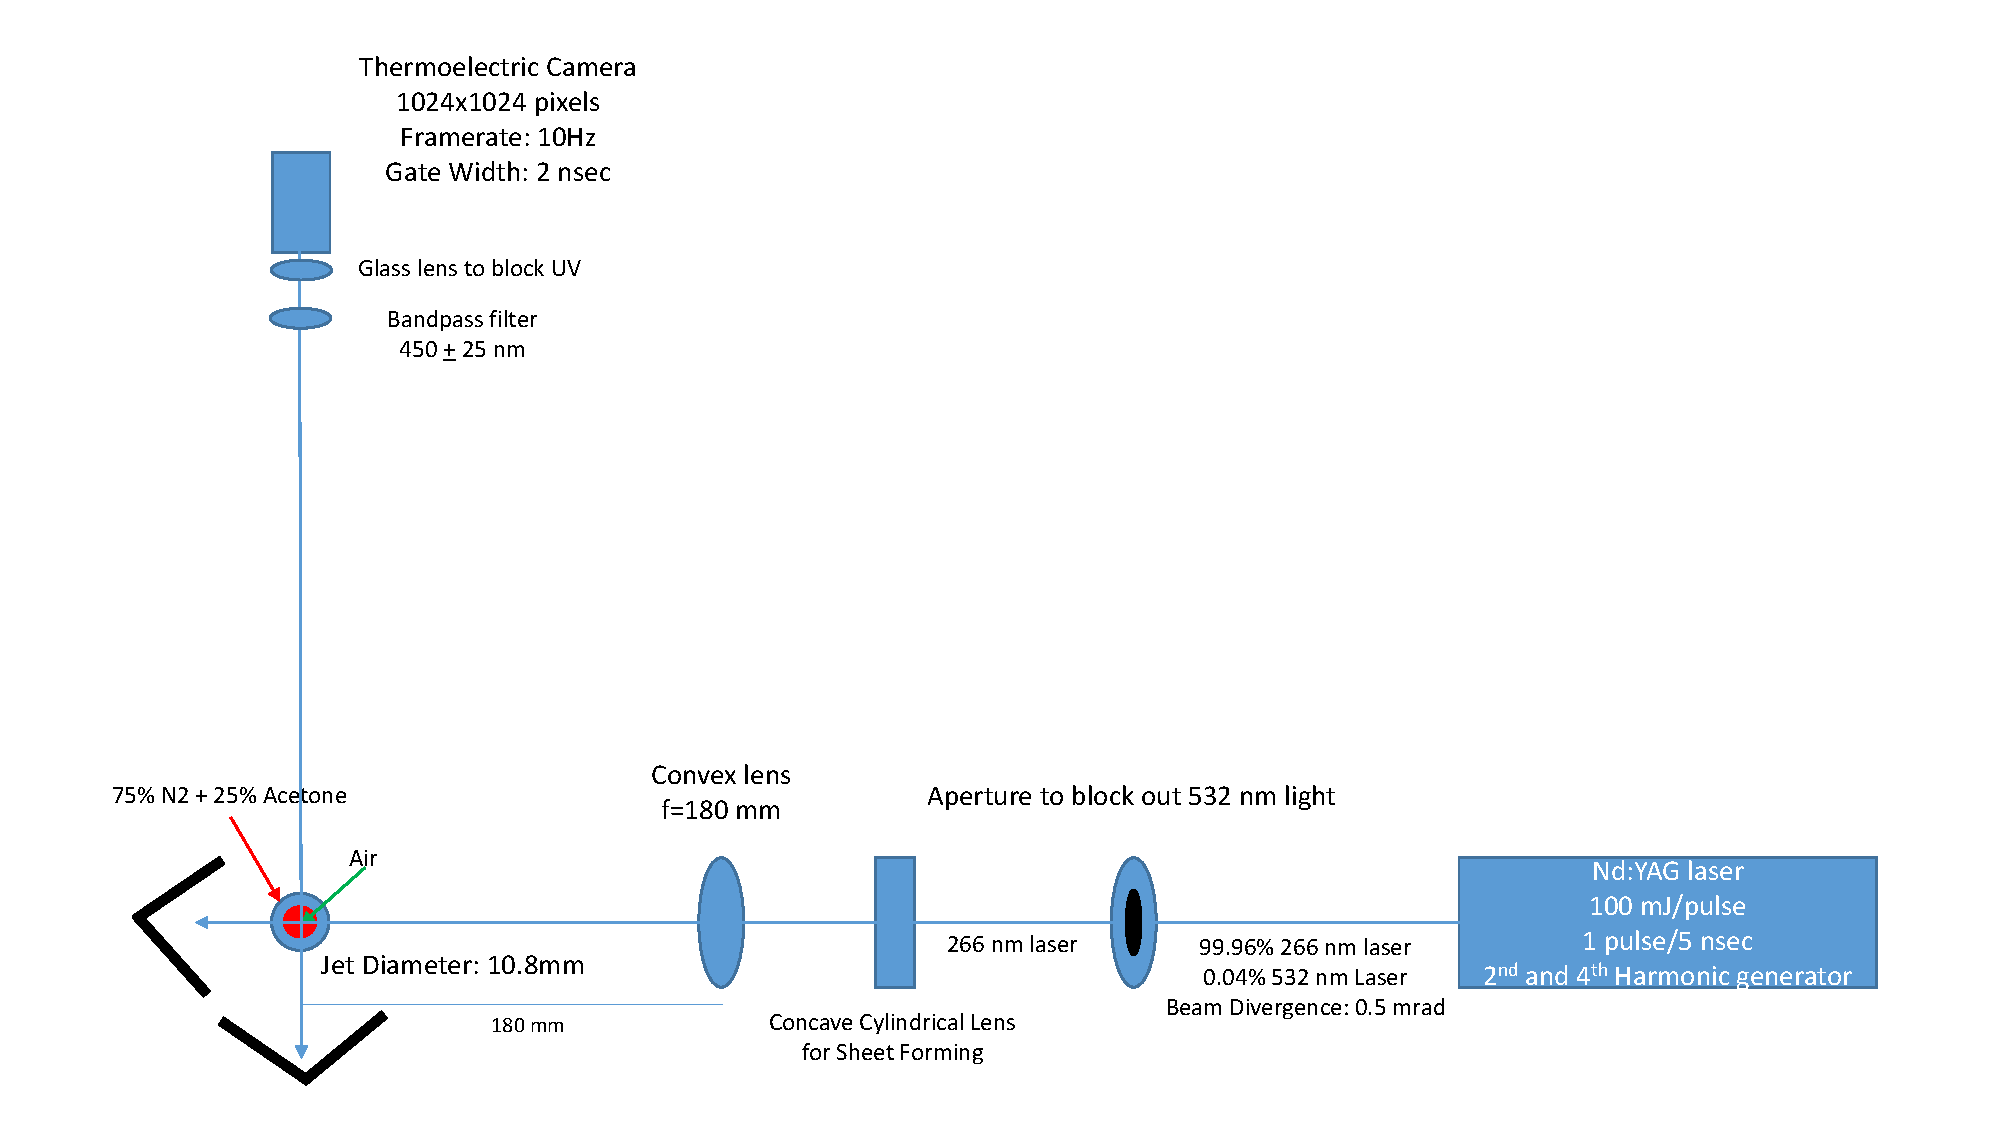
\includegraphics[width=\linewidth]{Lab3Diagram.pdf}
    \caption{{\footnotesize PLIF Lab Setup}}
\end{figure}

This experiment was set up as shown in Figure 1.  The ND:YAG laser produced a beam with a wavelength of 1064 nanometers.  After the second and fourth harmonic generators, there will be three beams of wavelengths 1064 nanometers, 532 nanometers, and 266 nanometers.  As the beam leaves the laser body, the beam makeup will be as shown in figure 1.  The laser is aligned below the plane of the optical instruments, and so is bounced between two mirrors so that the laser beam is aligned with the instruments.    The laser beam then passed through an aperture whose diameter was set to prevent any 532 nanometer light from passing through.  This was accomplished by placing a piece of paper on the other side of the aperture.  The 532 nanometer light looked green on the light and the 266 nanometer light looked blue.  The blue light formed a small circle in the center of a larger green circle, so the aperture was slowly closed until only the blue light could be seen.  The beam next passed through a cylindrical lens that turned changed the laser beam into a vertical laser sheet.  Next the beam passed through a focusing lens with a focal length of 180 millimeters, and the lens was placed 180 mm from the jet. The laser then passed through the jet of acetone-seeded air, which led to LIF of the acetone.  After the laser passed through the jet, it was directed into a light blocker to end the laser beam.  The camera was focused so that the point at which the laser passed through the jet was in focus.  There was a black light block placed in the cameras view so that only fluorescence from the jet was detected by the camera and outside signals were minimized.  \newline
\indent This experiment was carried out four times, for two different Reynold's numbers and two different percentages of acetone in the jet at each reynold's number: 7500 and 5000, and 2\% and 2.5\% respectively.  At 5000 reynolds number, the total flowrate was calculated to be 1.48 SCFM and 2.21 SCFM and 7500.  The buffer gas flowrate was calculated by multiplying the percentage of acetone by 4 then multiplying that value by the total.  This could be done because it was known that the acetone to N2 ration was 1:3.  This gave buffer gas flowrates of 0.1184 SCFM and 0.148 SCFM at 2\% and 2.5\% at Re=5000 and 0.1768 SCFM and 0.221 SCFM at 2\% and 2.5\% at Re=7500.  These values were adjusted using a flow rate apparatus where the flowrate through a pipe was measured and adjusted using a valve. \newline
\indent Focusing the camera required removing the bandpass filter and focusing on a piece of paper that was placed on the jet.  The bandpass filter was reattached, which changed the focusing a negligible amount.  Next, the spatial resolution of the camera was calculated.  To do this, a piece of paper with two marks 2 cm apart was placed in the center of the jet's opening.  Then, the focused camera took an image at that position and the number of pixels between the two marks were found and used to calculate the resolution.  It was found that the distance between the two marks was 286 pixels, which gave a value of 14.3 pixels per millimeter. \newline
\indent For the experiment, the camera took 100 images at each reynold's number and percentage of acetone and these images were viewed using a computer program that gave information about the image.  This program was able to generate an averaged image of the 100 images.  A data set was generated by the program at various distances from the bottom of the image, with the distance being determined by the equation $y=\frac{x}{D}$ where D was the diameter of the jet, y is the distance above the jet where the images were taken, and x was given the value of 2, 4, and 6, resulting in 3 sets of images at each reynold's number and percent acetone.  First, a background image was taken with no jet being run, and the program removed these values from the subsequent ones with the jet running. \newline
\indent The program used to analyze the gathered images gave an intensity reading for each image, and was able to export all of this information as an Excel file.  The intensity is a proportional to the concentration due to the linearity of PLIF as a measurement tool.  This data was all taken at ambient temperature of 19\degree C and 100.2032 kPa.
$$$$
\begin{center}
    \section*{Results and Discussion}
\end{center}
As can be seen from Figures 2-13, within a reynold's number group and a concentration group, as the distance from the the jet orifice increased, the intensity decreased and the distance the jet was spread over increased.  As the concentration changed within a constant Reynold's number group, the intensity increased and the distance the jet was spread over stayed approximately the same.  As the Reynold's number increased from 5000 to 7500, the intensity increased and the distance the jet was spread over stayed approximately the same. These results were all as expected.  It should be noted that the dip seen to the right of the peak of the intensity graphs is unexpected, but is likely due to a physical blockage or deformation in the jet orifice.\newline
\indent Figures 14-29 show three sample images and one averaged image for each reynold's number and concentration.  As expected, the jet began fairly compactly but then spread out as it moved further away from the orifice.  These images reinforce the interpretation of firgures 2-13 as discussed above. 
\indent In order to estimate the radius of the jet, the distance between the maximum intensity data point and the beginning of the jet was calculated using the different data sets.  Then, the average value of these radii was calculated to be 0.57 inches.  This is a fairly large divergence from the results from LIF and absorption, 0.65 inches and 0.62 inches respectively.  Any discrepancy between these values is likely due to imperfect measurements or data analysis.  For example, the maximum intensity point in the data sets used to get the PLIF radius may not correspond to the exact center of the jet, which can be seen to be the case in many of the graphs below. \newline
\indent Sources of error include background noise, a slightly out of focus camera, possible alignment imperfections, assumption of ideal optical instruments, and human error in calculations.  Background noise was minimized by taking a background image at the beginning of the experiment, but could be minimized further by taking a background image between every test run.  Any potential alignment issues could be dealt with by incorporating a more precise apparatus.  It could be possible to minimize human error by finding a more precise way of estimating the radius rather than physically looking at data and guessing where the jet began.  One large potential source of error was the line that ran through all of the images, as can be seen in the images below, particularly in the averaged images.  It is unknown what caused this line, but an experiment that did not include this would likely be more accurate. 


\newpage
\begin{center}
    \section*{References}
\end{center}
\newline
\textbf{1)} Lee, \textit{"Chapter 4: Laser Induced Fluorescence"}, University of Cincinnati Class Notes, Fall 2019 \newline
\textbf{2)}  A. Lozano, B. Yip, and R. K. Hanson, “Acetone: a tracer for concentration measurements in gaseous flows by planar laserinduced fluorescence,” Exp. Fluids 13, 369–376 (1992) \newline
\textbf{3)}  Lucinda S. Yuen, James E. Peters, and Robert P. Lucht, "Pressure dependence of laser-induced fluorescence from acetone," Appl. Opt. 36, 3271-3277 (1997)\newline
\textbf{4)}  Mark C. Thurber, Frédéric Grisch, and Ronald K. Hanson, "Temperature imaging with single-and dual-wavelength acetone planar laser-induced fluorescence," Opt. Lett. 22, 251-253 (1997) \newline
\textbf{5)} M. C. Thurber and R. K. Hanson, "Pressure and composition dependences of acetone laser-induced fluorescence with excitation at 248, 266, and 308 nm," Appl. Phys. B 69, 229-240 (1999) \newline
\textbf{6)} Gabriel Laufer, \textit{Introduction to Optics and Lasers in Engineering}, Cambridge University Press, (1996) \newline
\newpage
\begin{center}
    \section*{Appendix}
    \subsection*{Data Analysis and Images}
\end{center}
\begin{figure}[h]
    \centering
    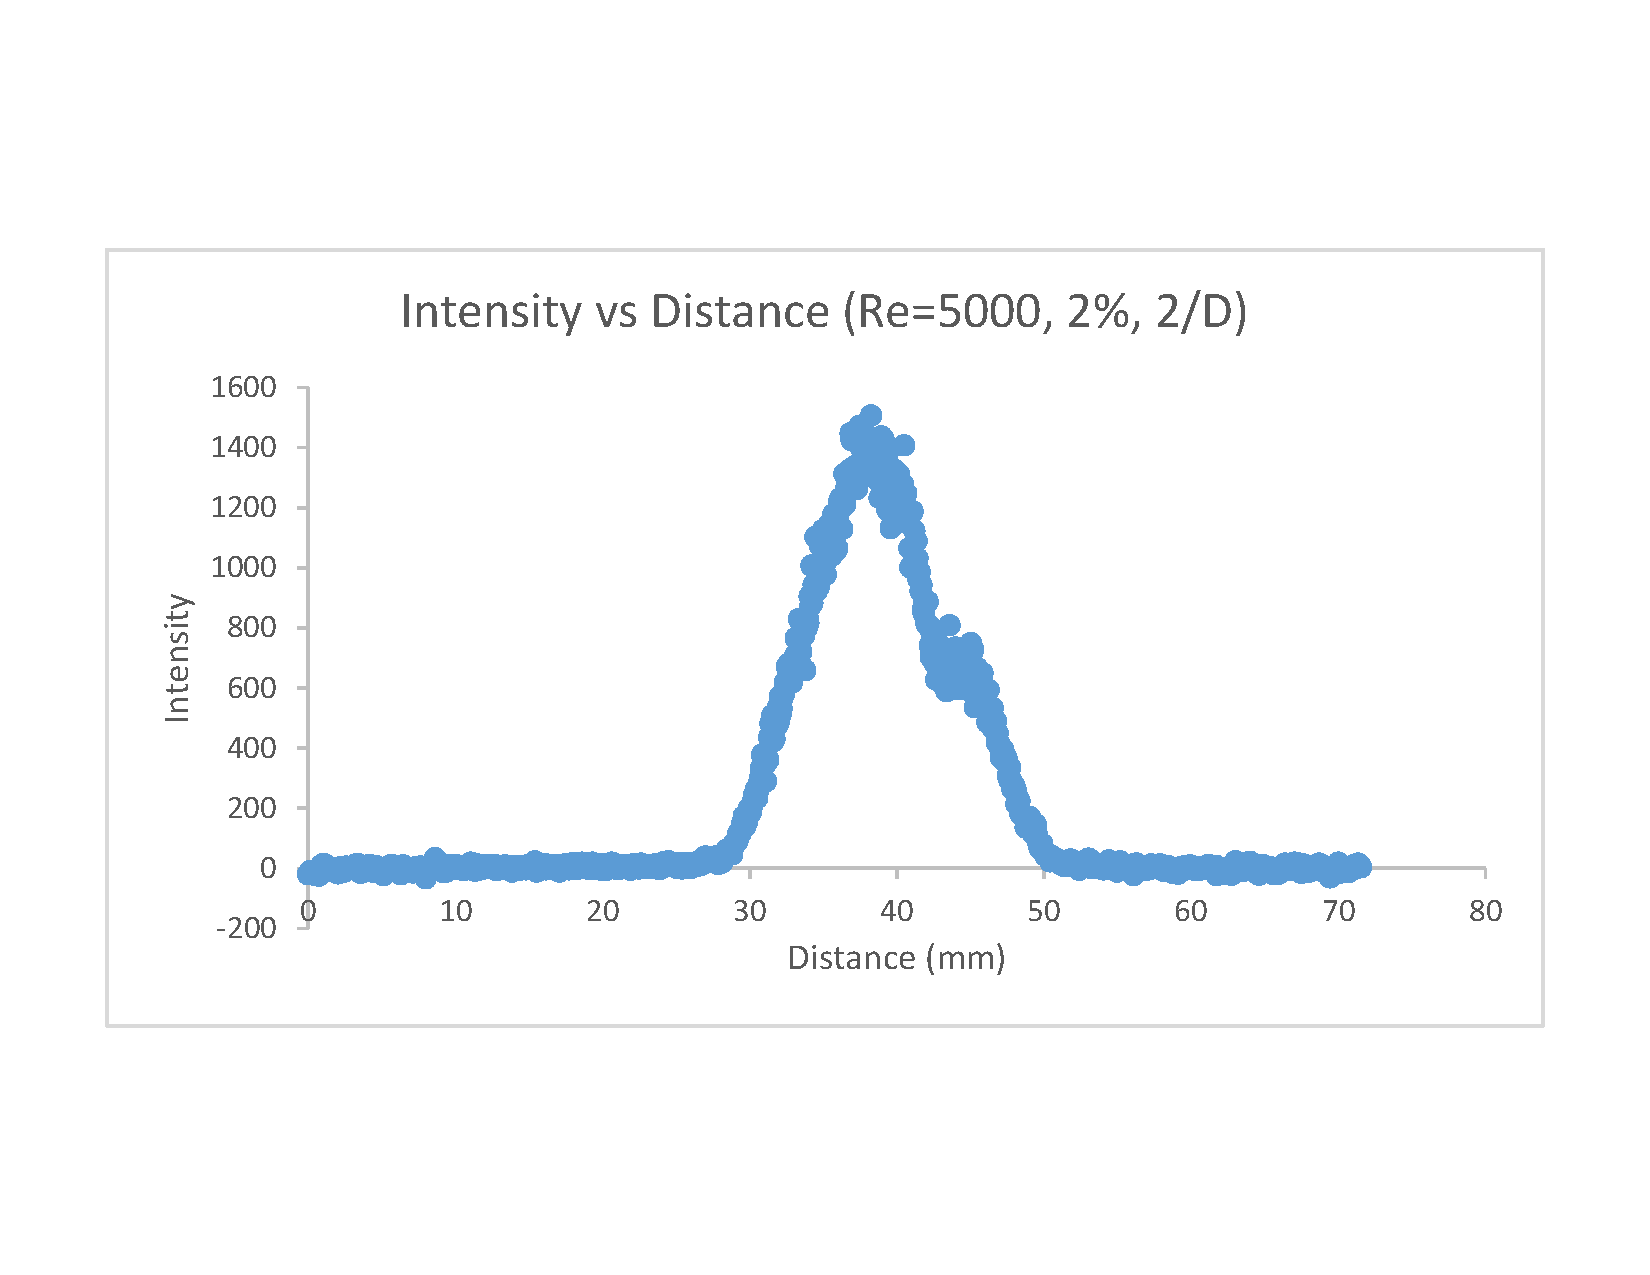
\includegraphics[width=0.55\linewidth]{RE-5000-20-cs2D.pdf}
    \caption{{\footnotesize Re=5000, 2\%, $\frac{2}{D}$ }}
\end{figure}
\begin{figure}[h]
    \centering
    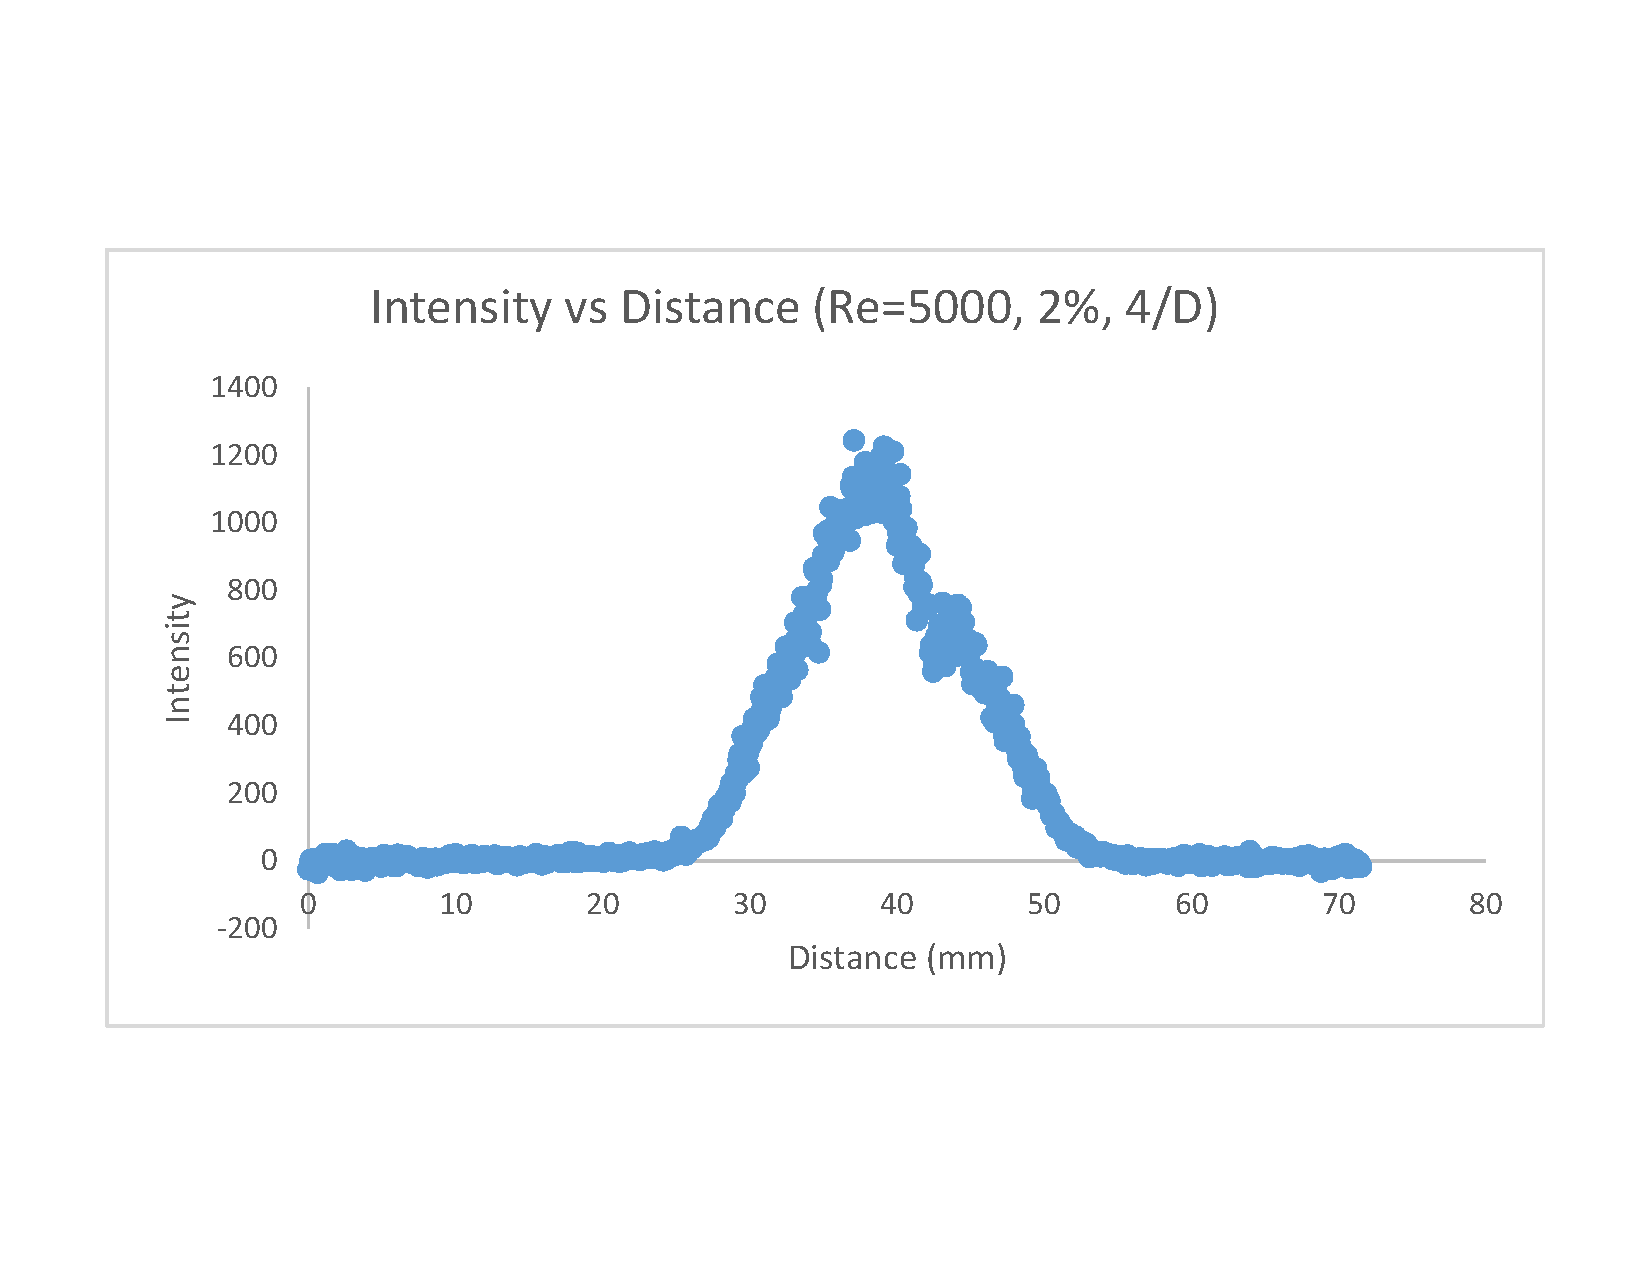
\includegraphics[width=0.55\linewidth]{RE-5000-20-cs4D.pdf}
    \caption{{\footnotesize Re=5000, 2\%, $\frac{4}{D}$ }}
\end{figure}
\begin{figure}[h]
    \centering
    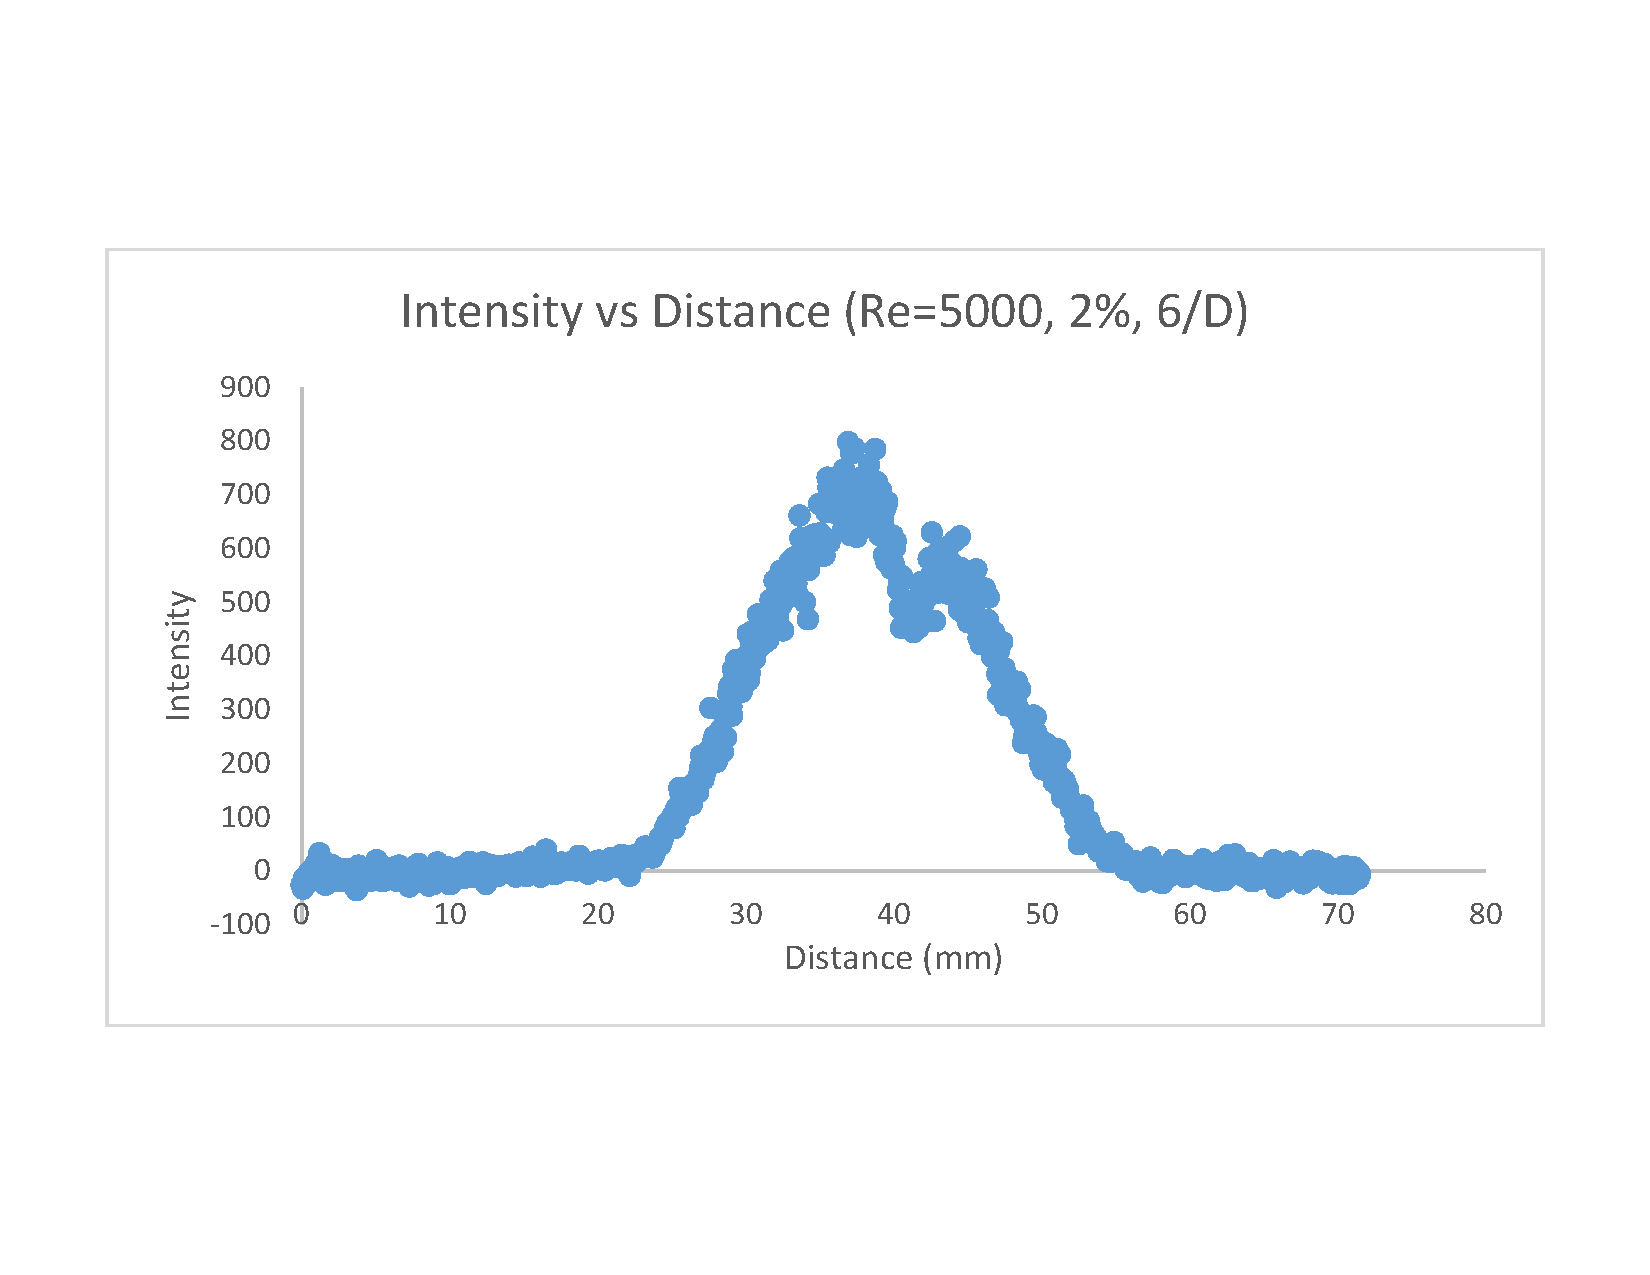
\includegraphics[width=0.55\linewidth]{RE-5000-20-cs6D.pdf}
    \caption{{\footnotesize Re=5000, 2\%, $\frac{6}{D}$ }}
\end{figure}
\begin{figure}[h]
    \centering
    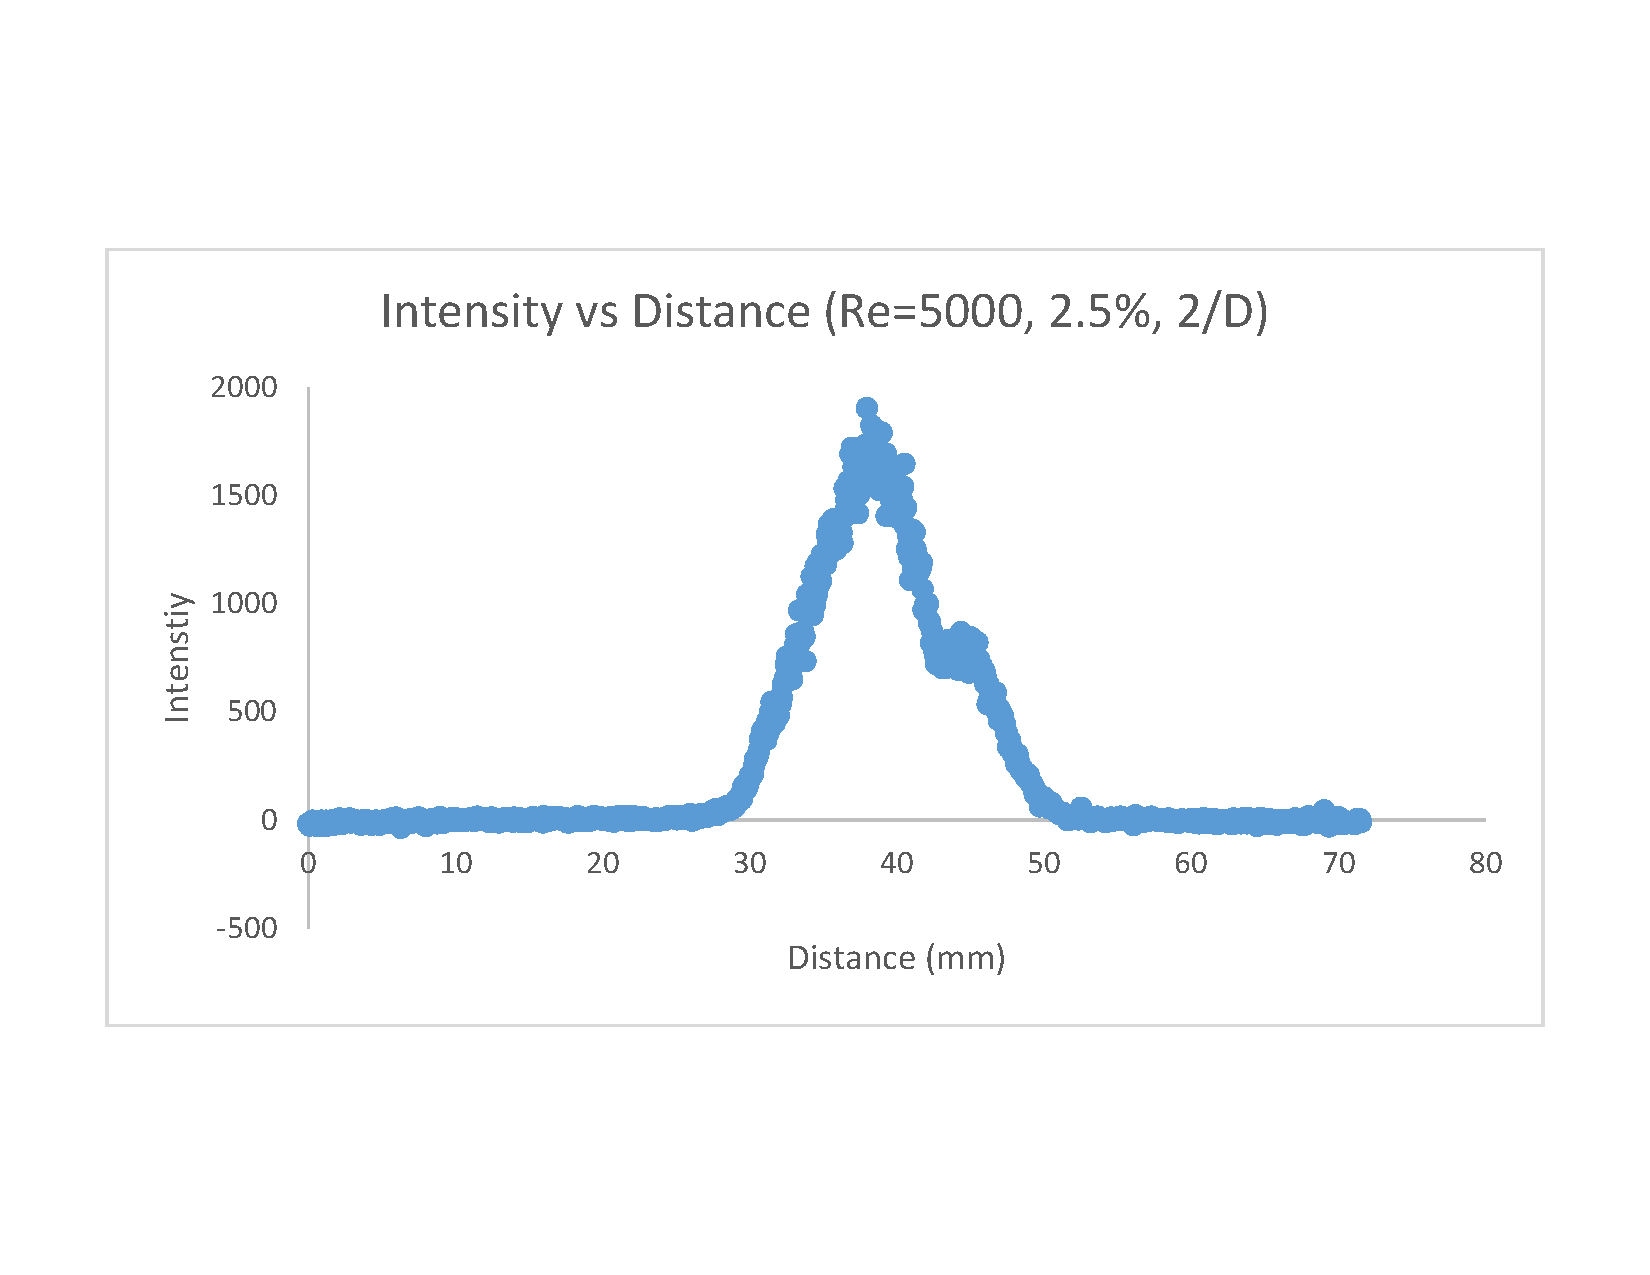
\includegraphics[width=0.55\linewidth]{RE-5000-25-cs2D.pdf}
    \caption{{\footnotesize Re=5000, 2.5\%, $\frac{2}{D}$ }}
\end{figure}
\begin{figure}[h]
    \centering
    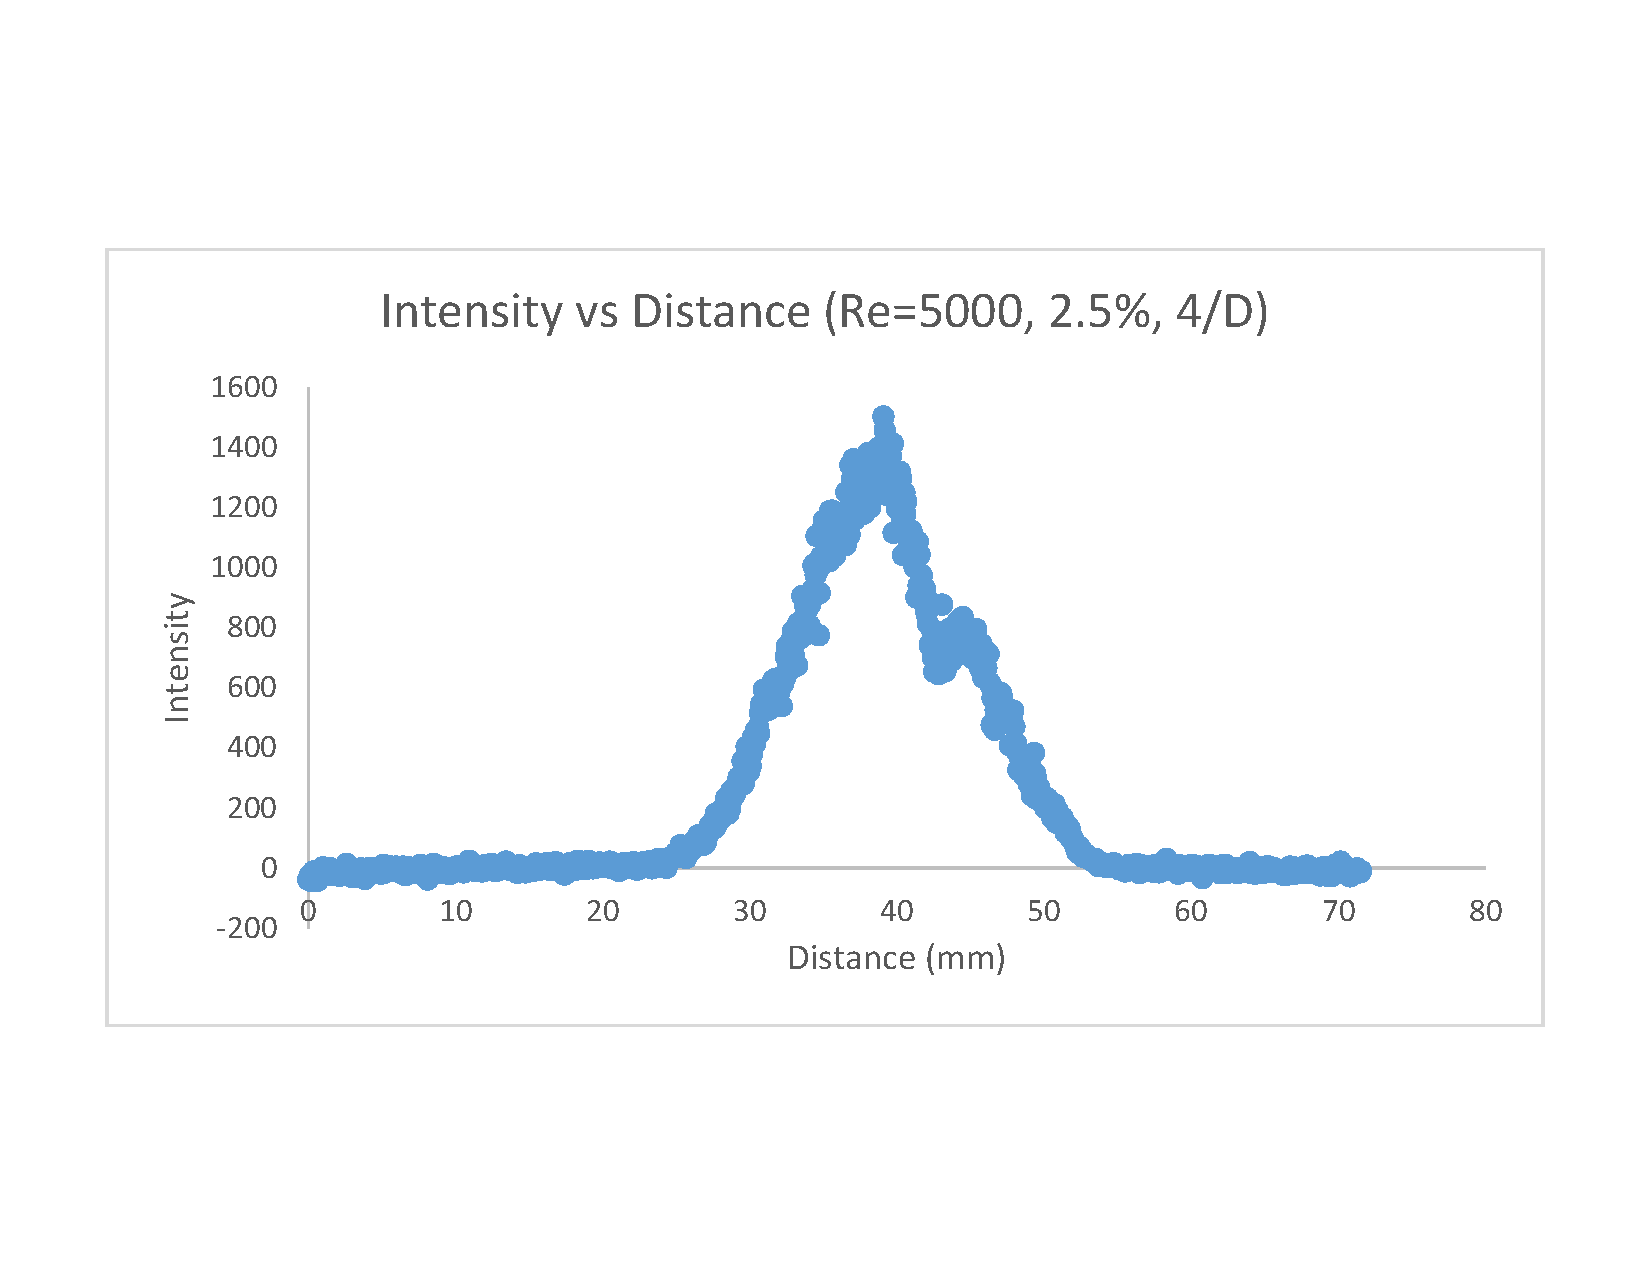
\includegraphics[width=0.55\linewidth]{RE-5000-25-cs4D.pdf}
    \caption{{\footnotesize Re=5000, 2.5\%, $\frac{4}{D}$ }}
\end{figure}
\begin{figure}[h]
    \centering
    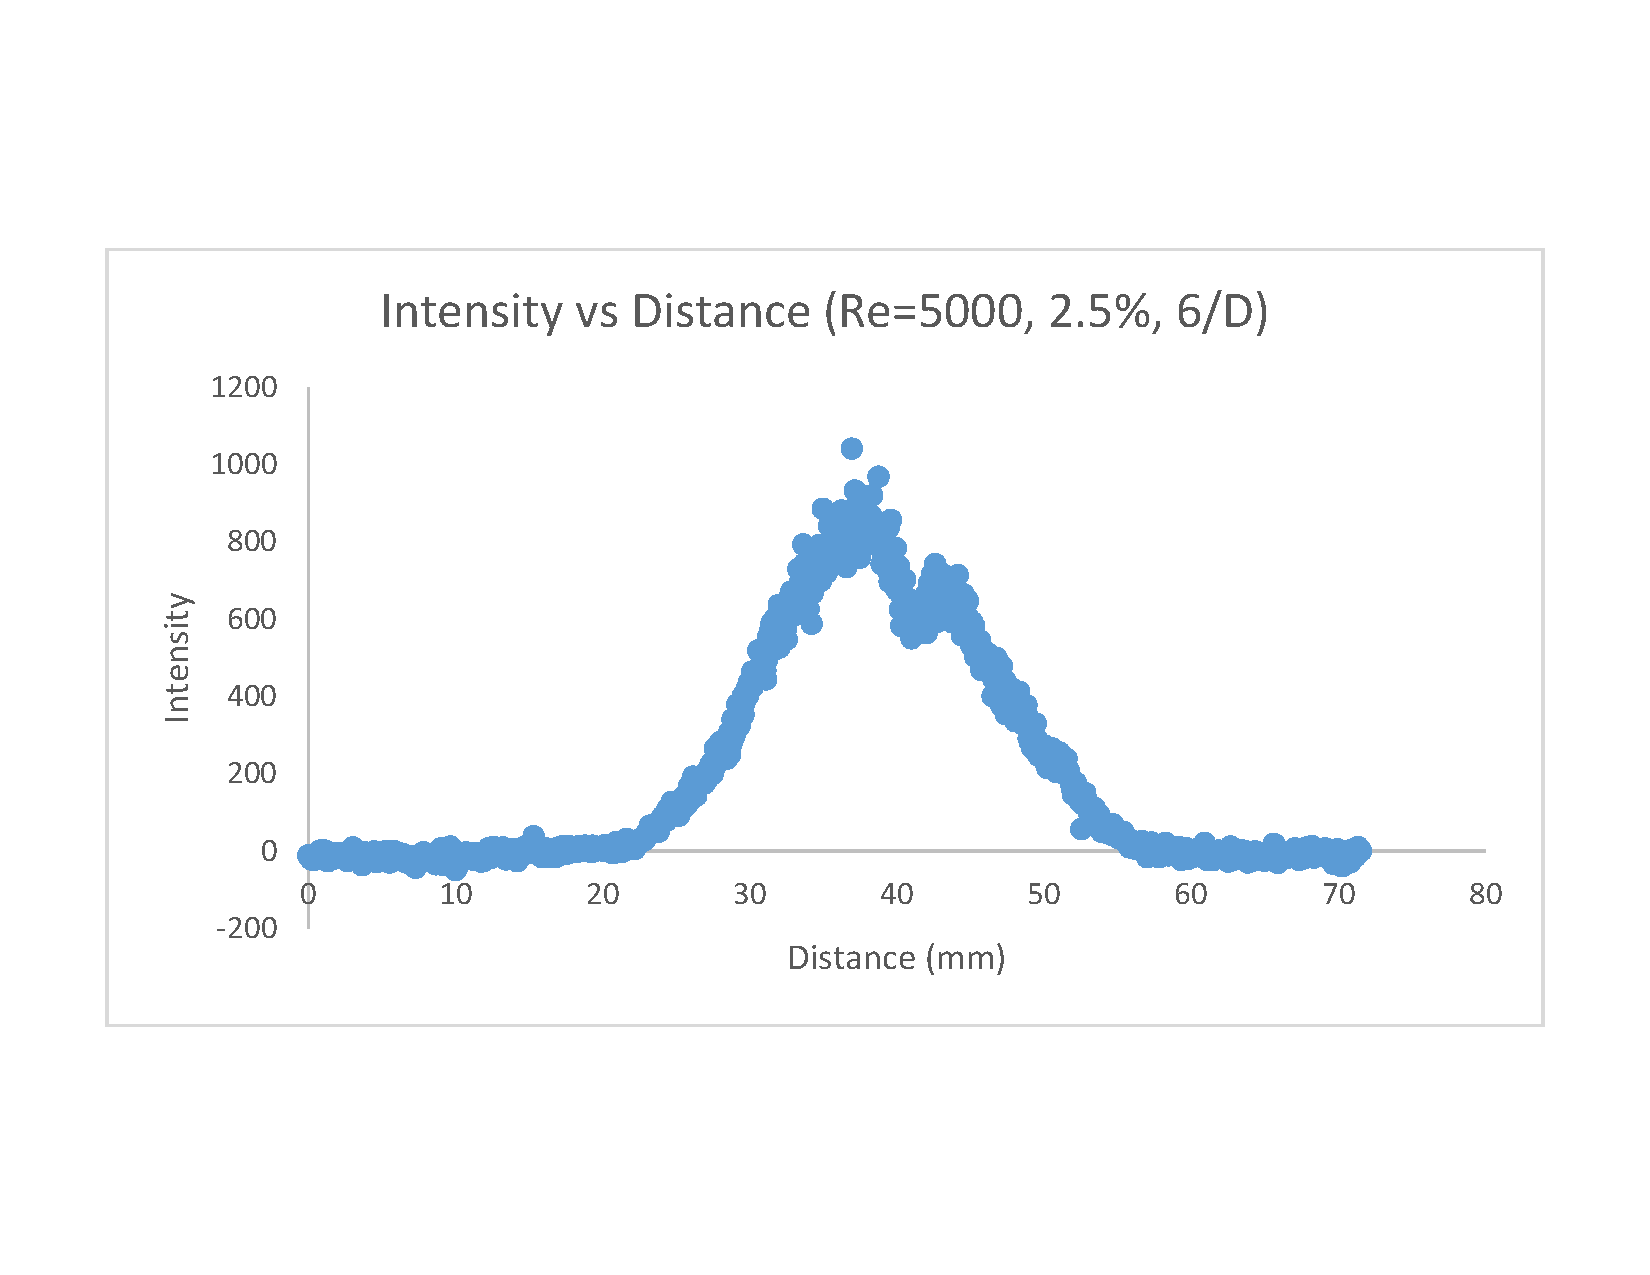
\includegraphics[width=0.55\linewidth]{RE-5000-25-cs6D.pdf}
    \caption{{\footnotesize Re=5000, 2.5\%, $\frac{6}{D}$ }}
\end{figure}
\begin{figure}[h]
    \centering
    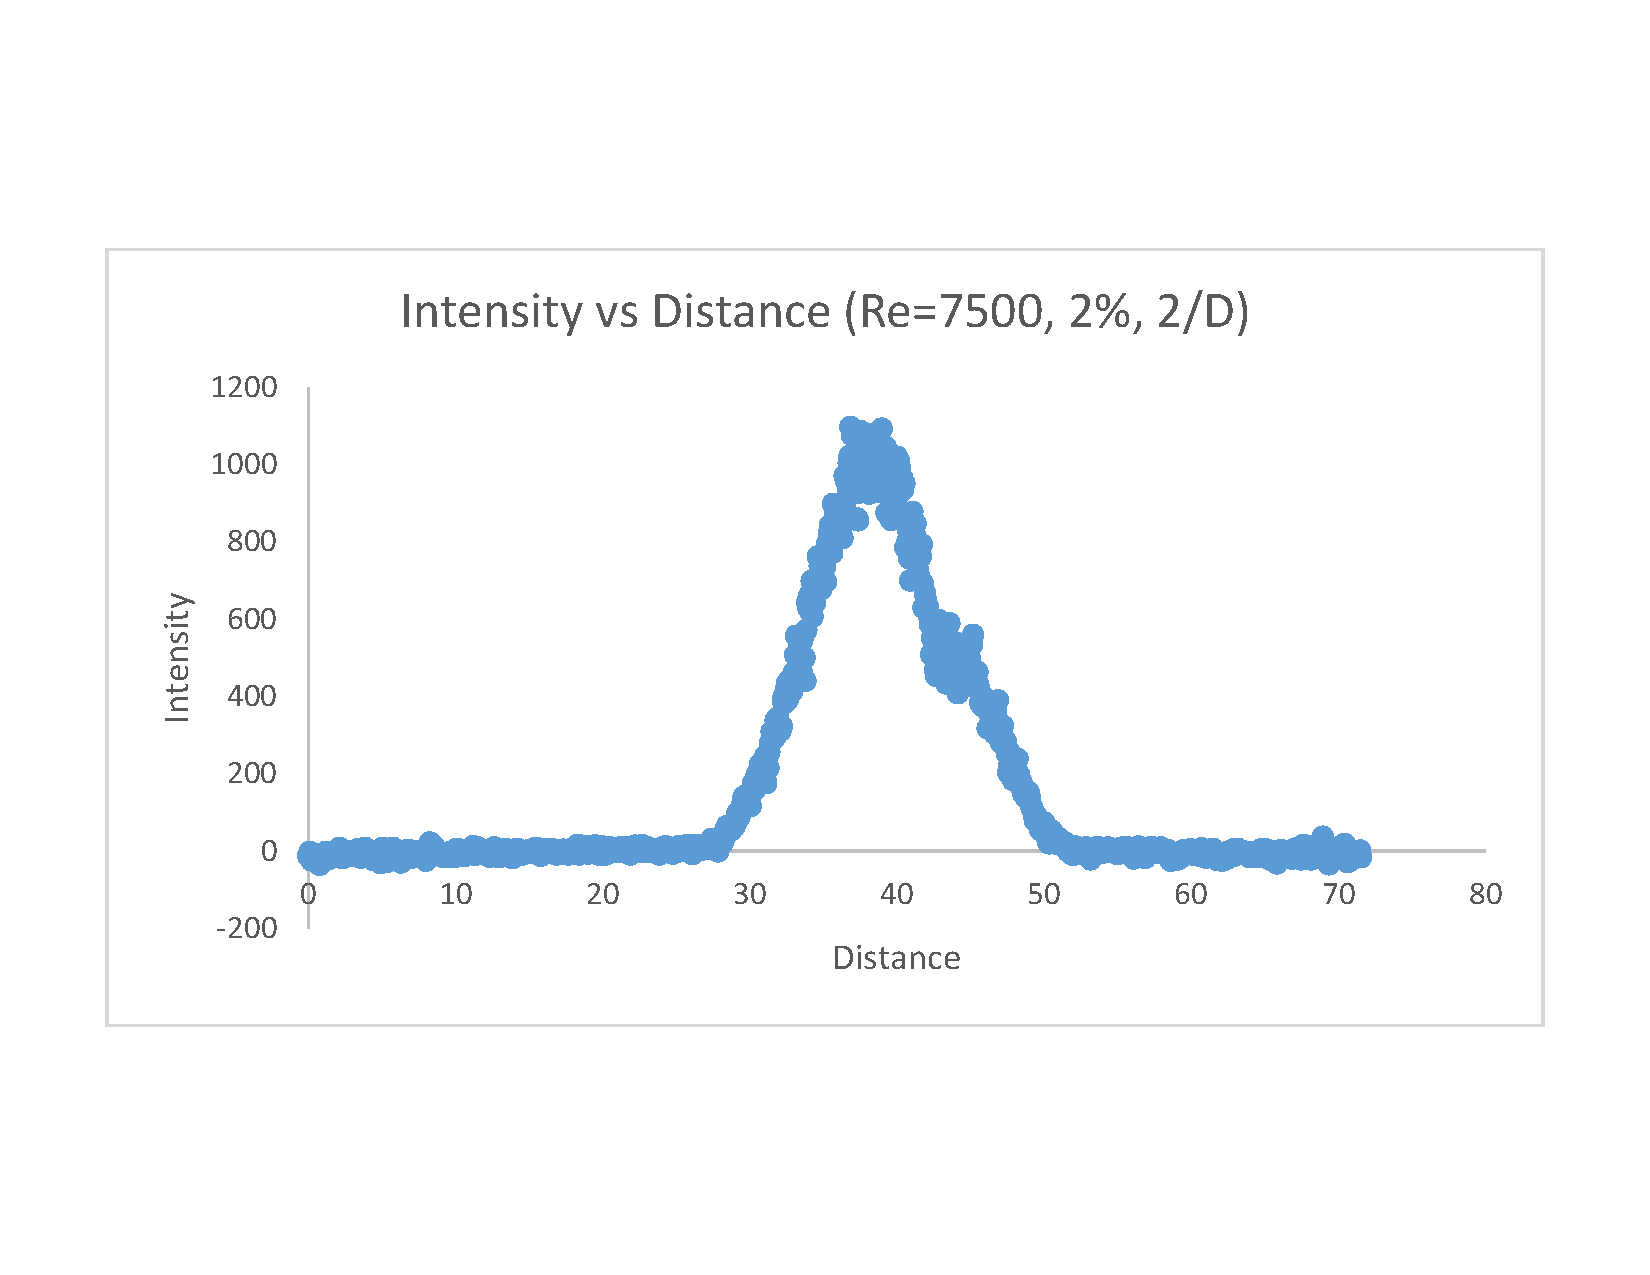
\includegraphics[width=0.55\linewidth]{RE-7500-20-cs2D.pdf}
    \caption{{\footnotesize Re=7500, 2\%, $\frac{2}{D}$ }}
\end{figure}
\begin{figure}[h]
    \centering
    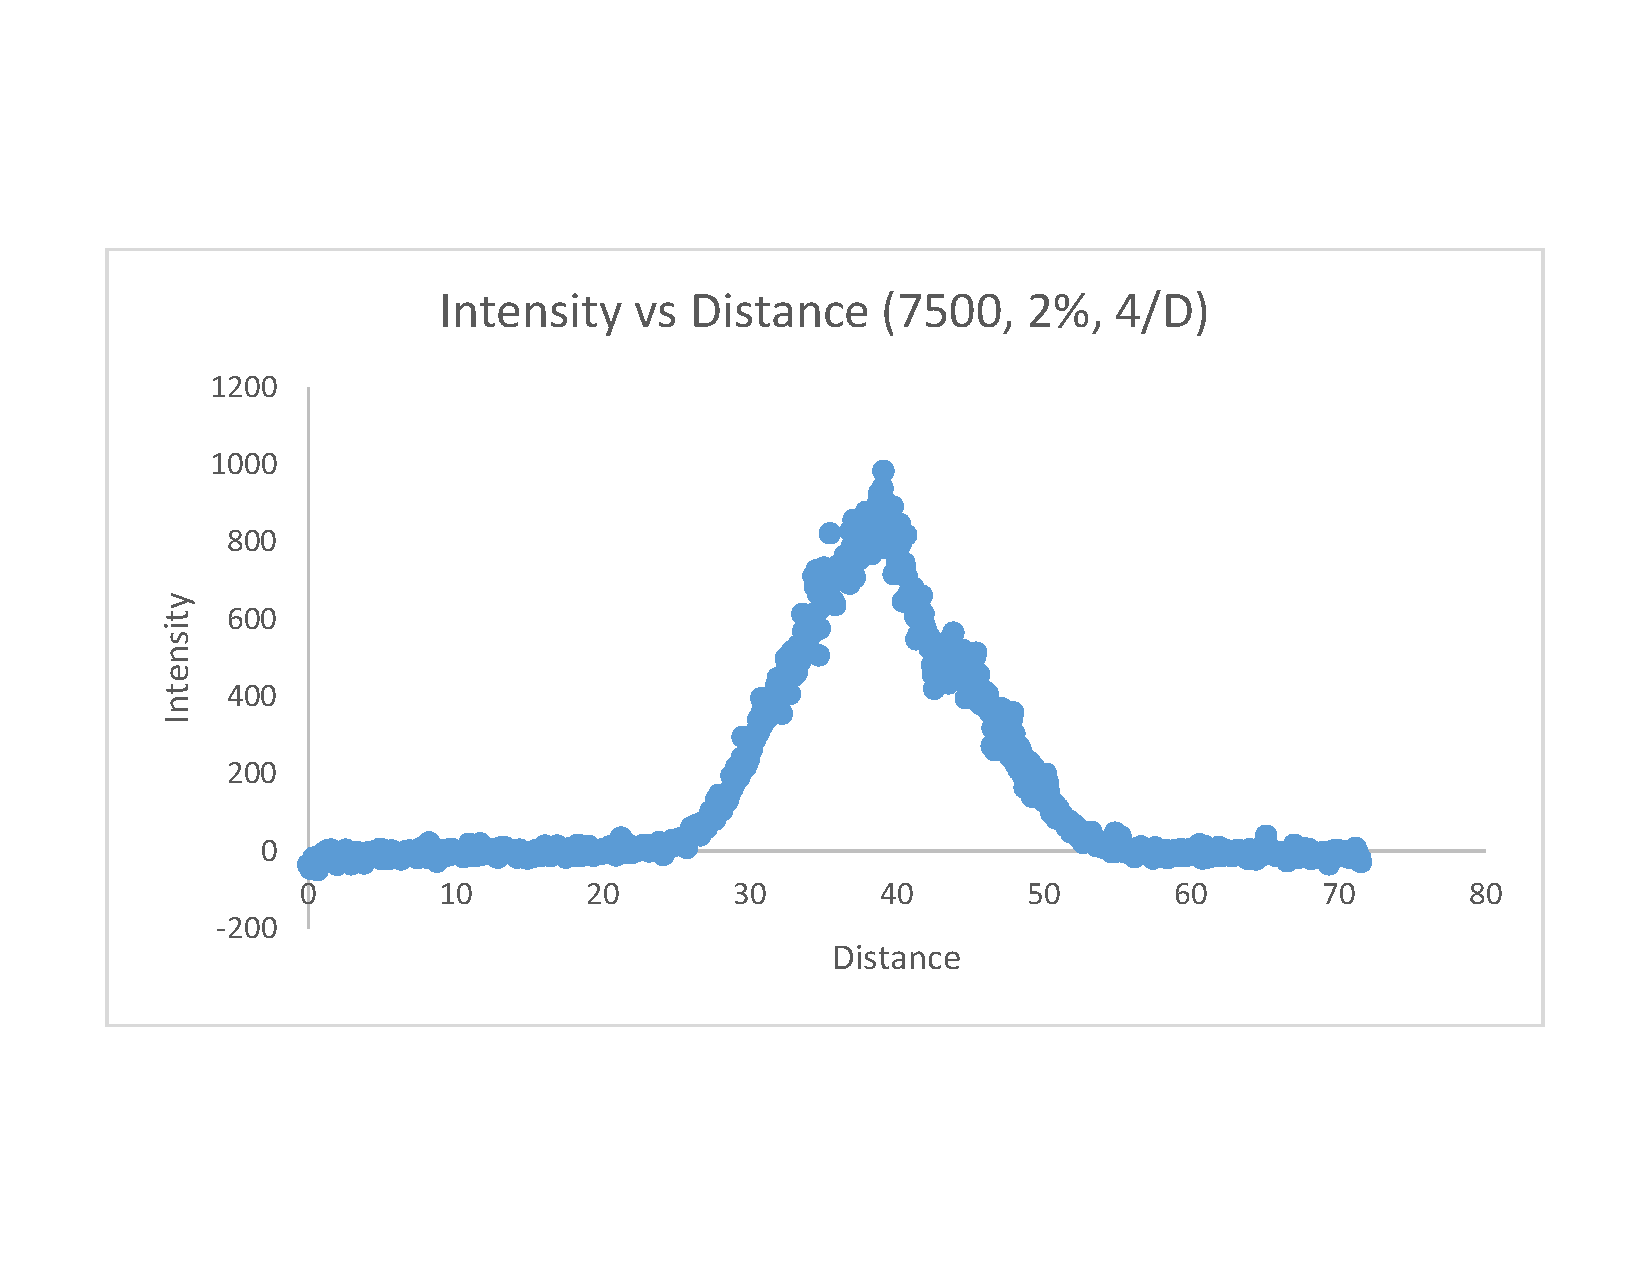
\includegraphics[width=0.55\linewidth]{RE-7500-20-cs4D.pdf}
    \caption{{\footnotesize Re=7500, 2\%, $\frac{4}{D}$ }}
\end{figure}
\begin{figure}[h]
    \centering
    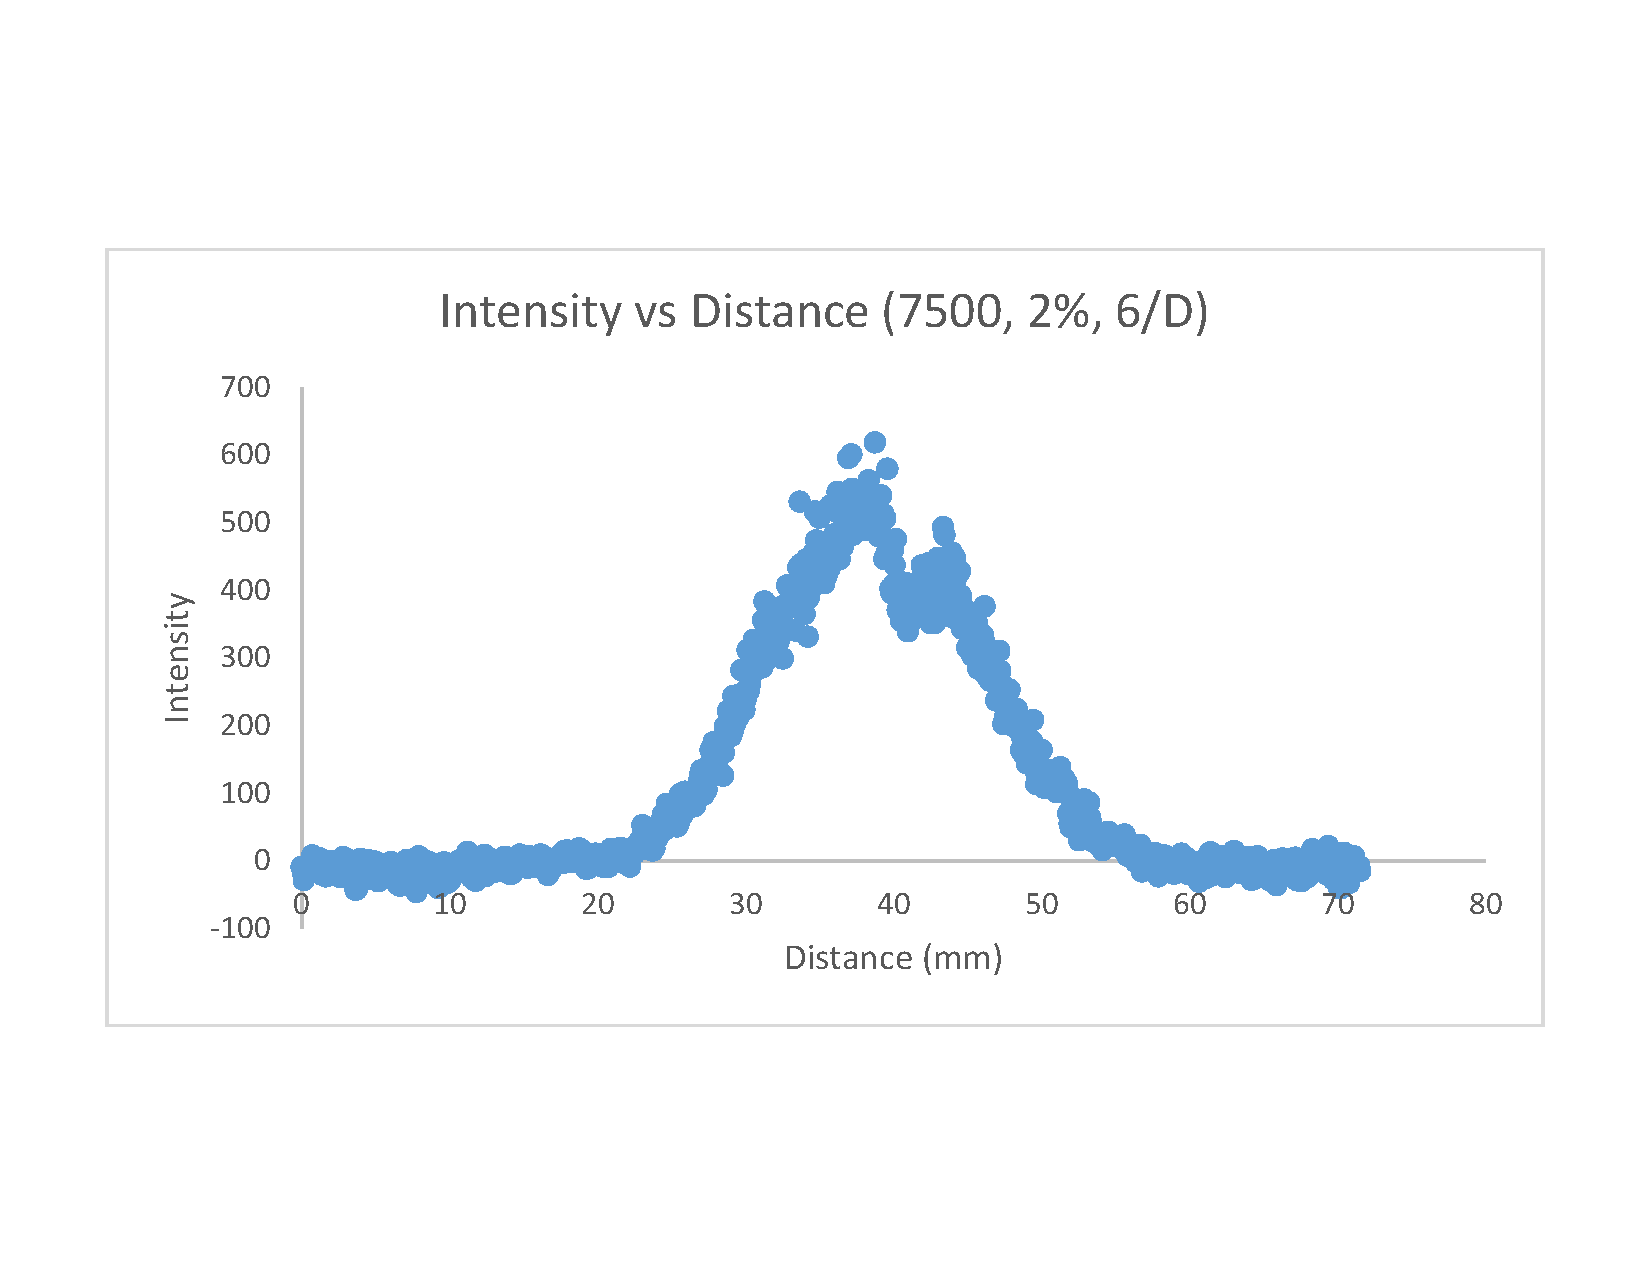
\includegraphics[width=0.55\linewidth]{RE-7500-20-cs6D.pdf}
    \caption{{\footnotesize Re=7500, 2\%, $\frac{6}{D}$ }}
\end{figure}\begin{figure}[h]
    \centering
    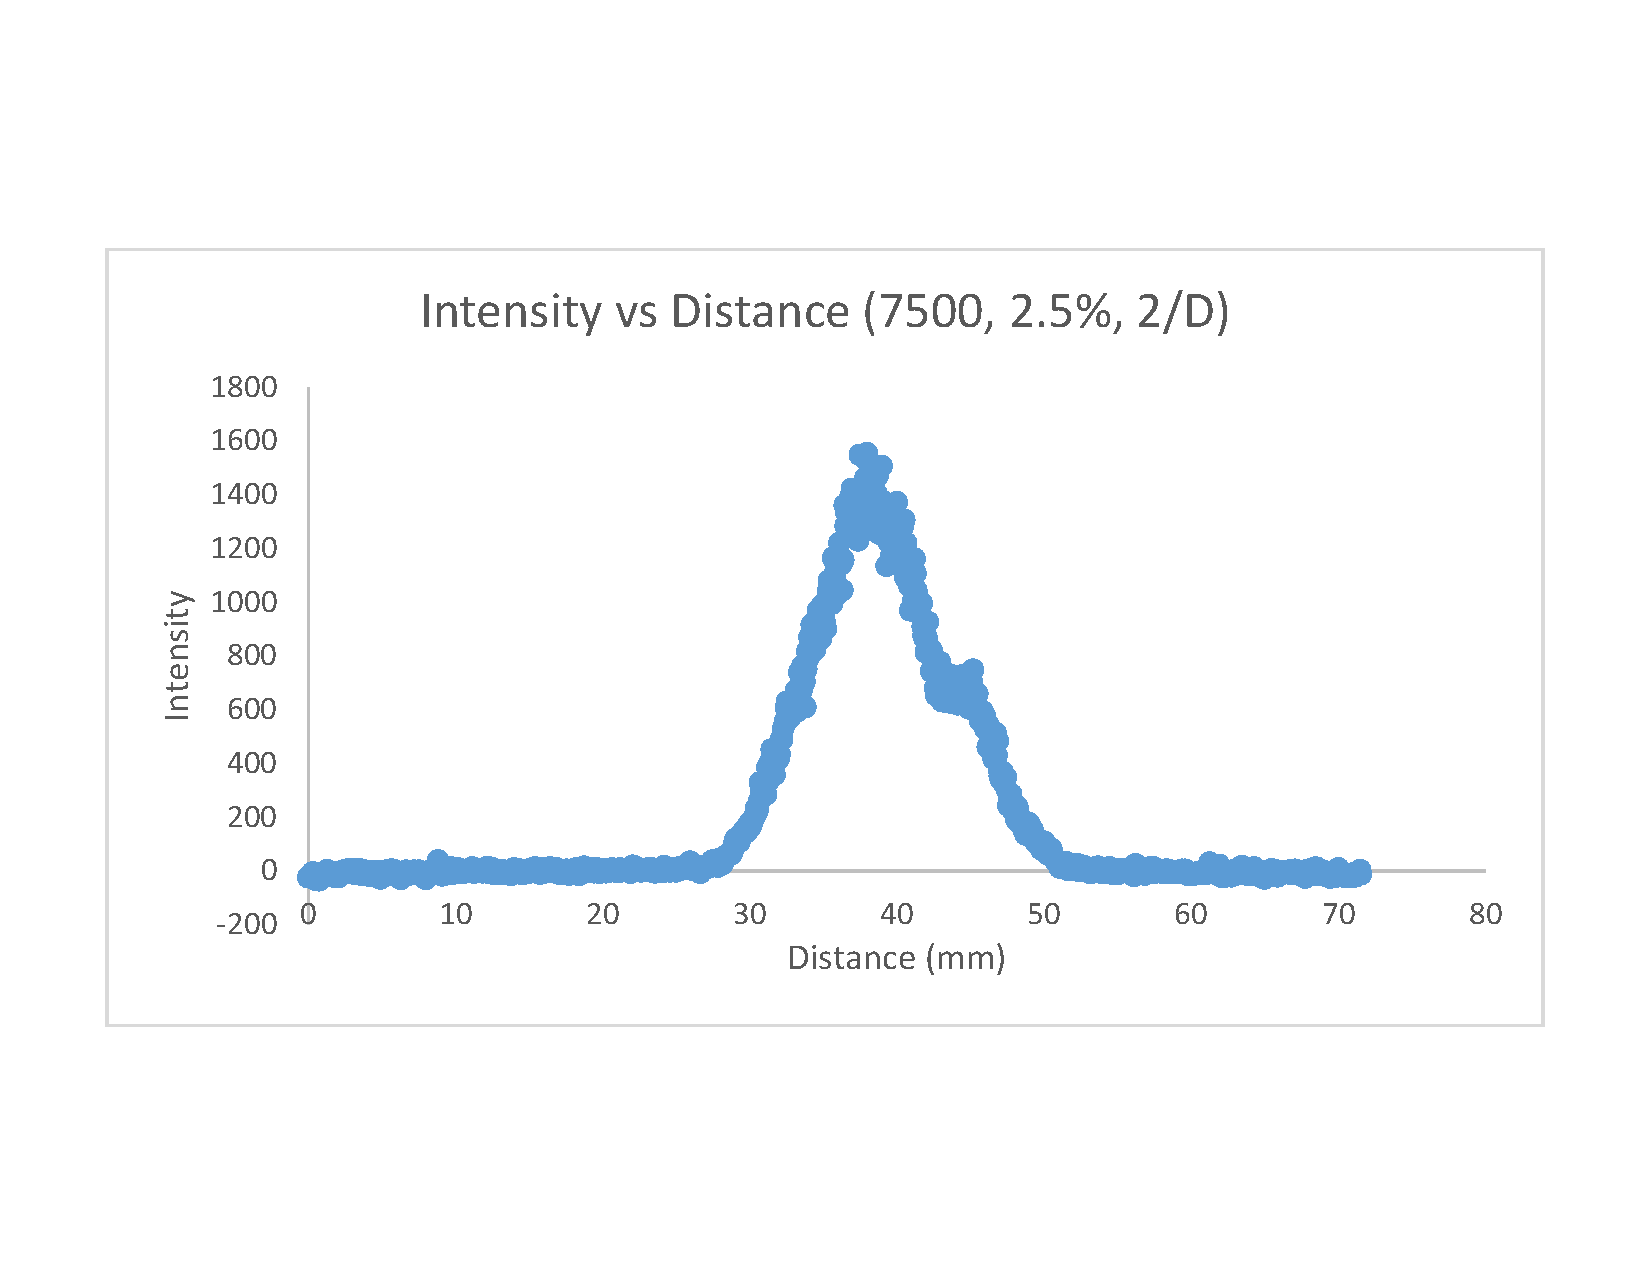
\includegraphics[width=0.55\linewidth]{RE-7500-25-cs2D.pdf}
    \caption{{\footnotesize Re=7500, 2.5\%, $\frac{2}{D}$ }}
\end{figure}\begin{figure}[h]
    \centering
    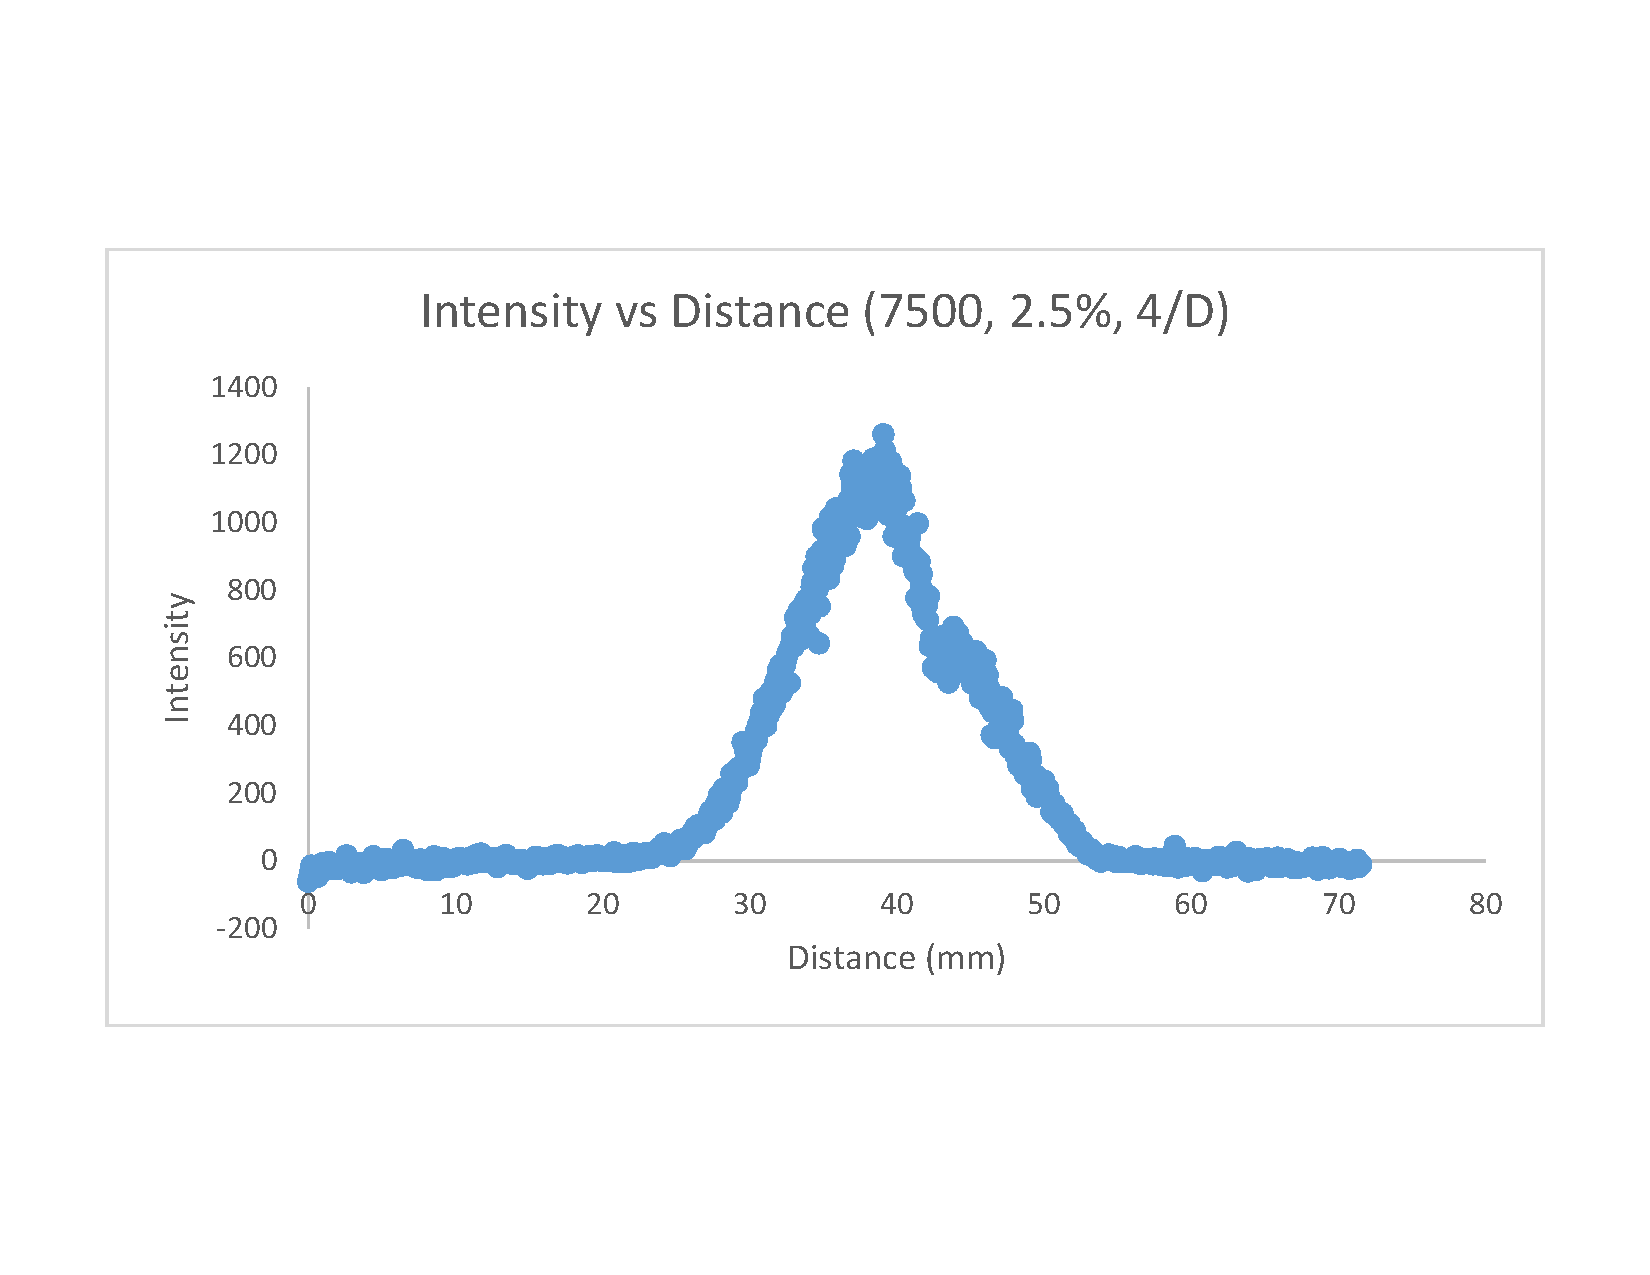
\includegraphics[width=0.55\linewidth]{RE-7500-25-cs4D.pdf}
    \caption{{\footnotesize Re=7500, 2.5\%, $\frac{4}{D}$ }}
\end{figure}
\begin{figure}[h]
    \centering
    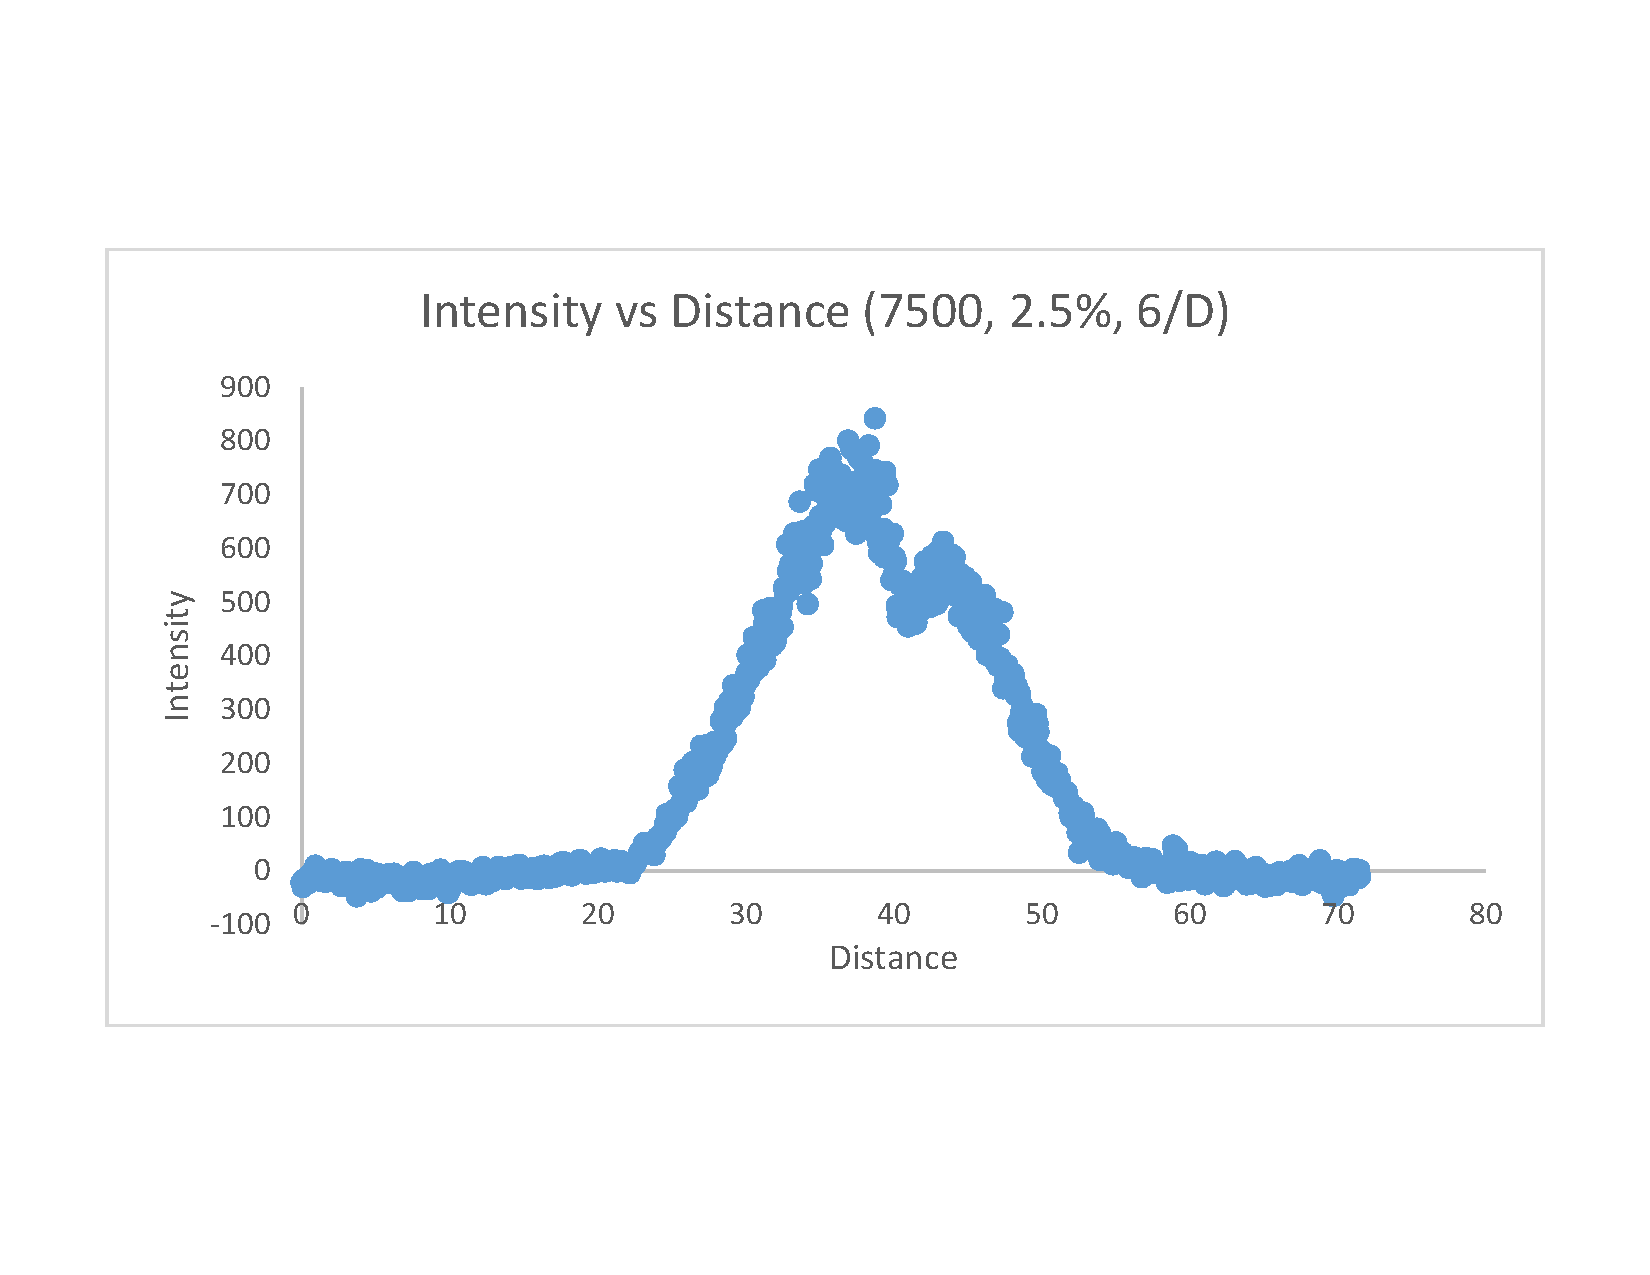
\includegraphics[width=0.55\linewidth]{RE-7500-25-cs6D.pdf}
    \caption{{\footnotesize Re=7500, 2.5\%, $\frac{6}{D}$ }}
\end{figure}

\begin{figure}[h]
    \centering
    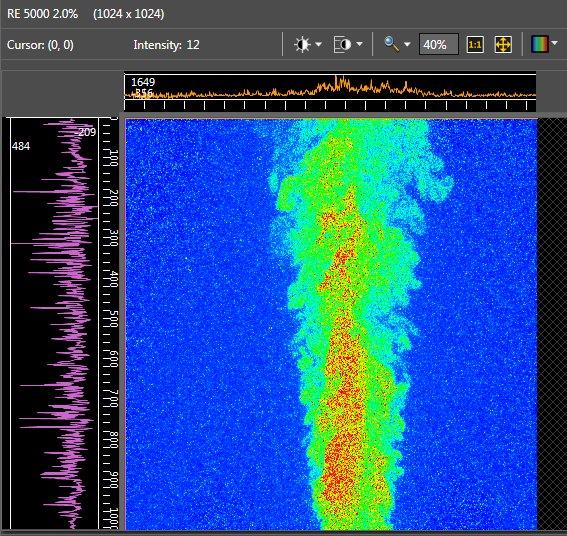
\includegraphics[width=0.55\linewidth]{RE-5000-20-1st.PNG}
    \caption{{\footnotesize Re=5000, 2.0\% Sample 1}}
\end{figure}
\begin{figure}[h]
    \centering
    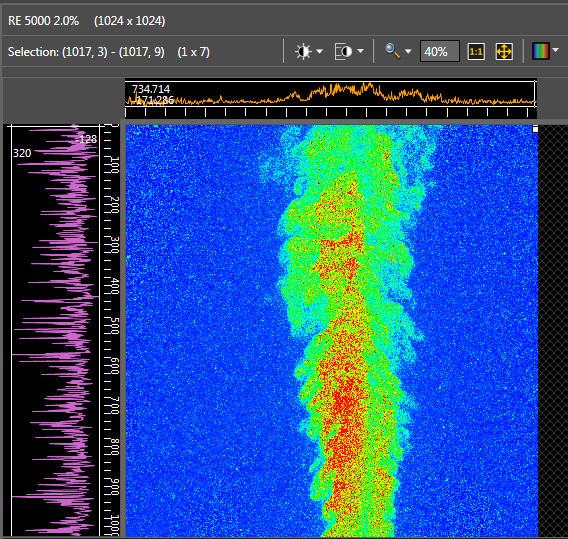
\includegraphics[width=0.55\linewidth]{RE-5000-20-2nd.PNG}
    \caption{{\footnotesize Re=5000, 2.0\% Sample 2}}
\end{figure}
\begin{figure}[h]
    \centering
    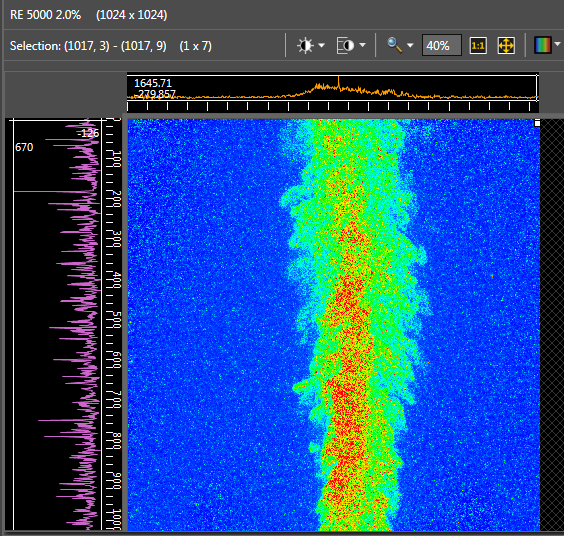
\includegraphics[width=0.55\linewidth]{RE-5000-20-3rd.PNG}
    \caption{{\footnotesize Re=5000, 2.0\% Sample 3}}
\end{figure}
\begin{figure}[h]
    \centering
    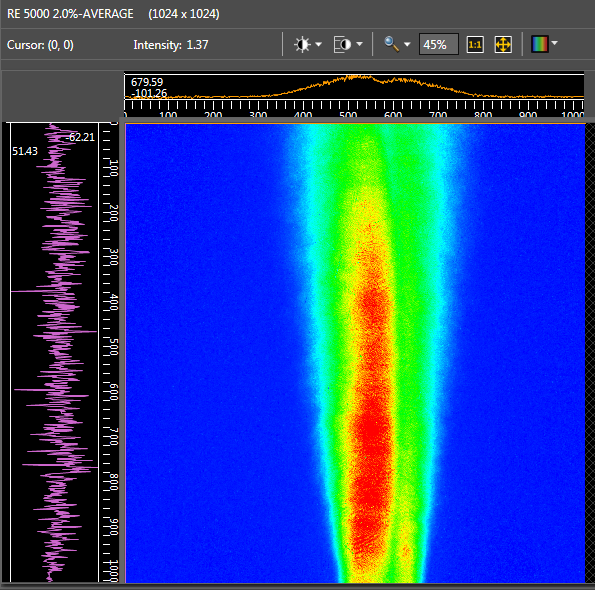
\includegraphics[width=0.55\linewidth]{RE-5000-20-Avg.PNG}
    \caption{{\footnotesize Re=5000, 2.0\% Average}}
\end{figure}

\begin{figure}[h]
    \centering
    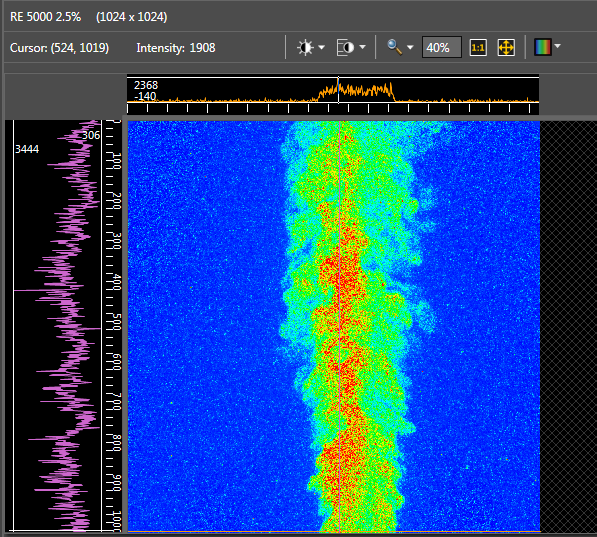
\includegraphics[width=0.55\linewidth]{RE-5000-25-1st.PNG}
    \caption{{\footnotesize Re=5000, 2.5\% Sample 1}}
\end{figure}
\begin{figure}[h]
    \centering
    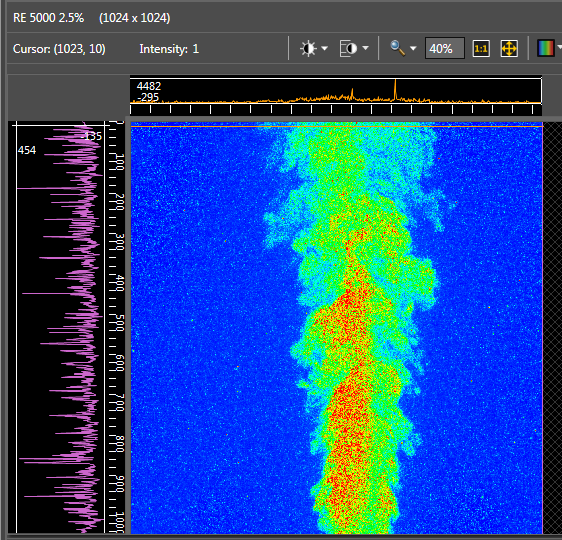
\includegraphics[width=0.55\linewidth]{RE-5000-25-2nd.PNG}
    \caption{{\footnotesize Re=5000, 2.5\% Sample 2}}
\end{figure}
\begin{figure}[h]
    \centering
    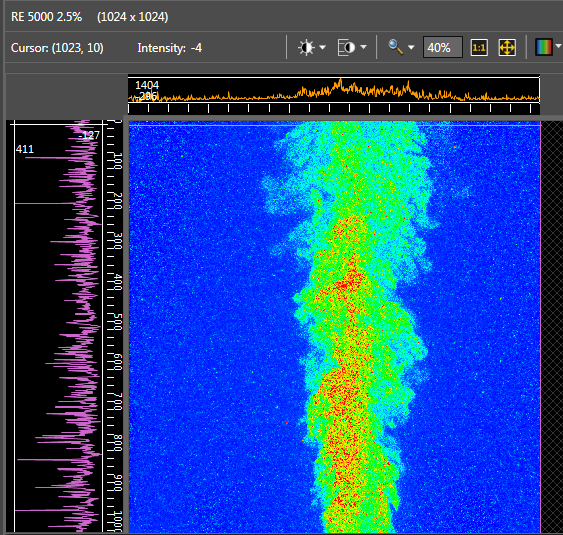
\includegraphics[width=0.55\linewidth]{RE-5000-25-3rd.PNG}
    \caption{{\footnotesize Re=5000, 2.5\% Sample 3}}
\end{figure}
\begin{figure}[h]
    \centering
    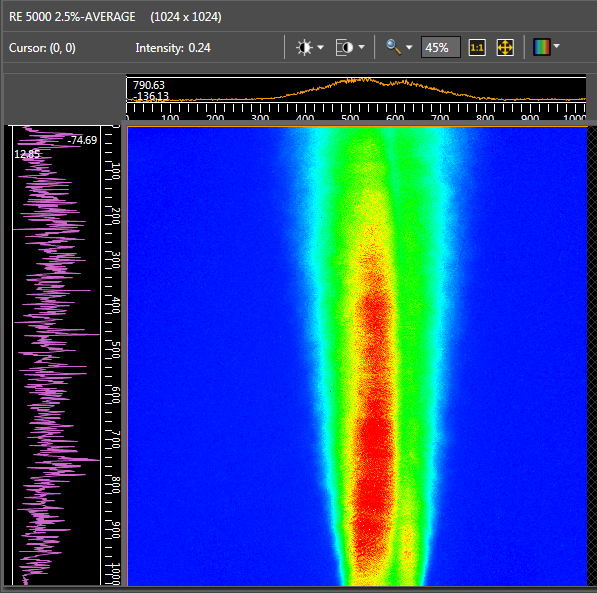
\includegraphics[width=0.55\linewidth]{RE-5000-25-Avg.PNG}
    \caption{{\footnotesize Re=5000, 2.5\% Average}}
\end{figure}

\begin{figure}[h]
    \centering
    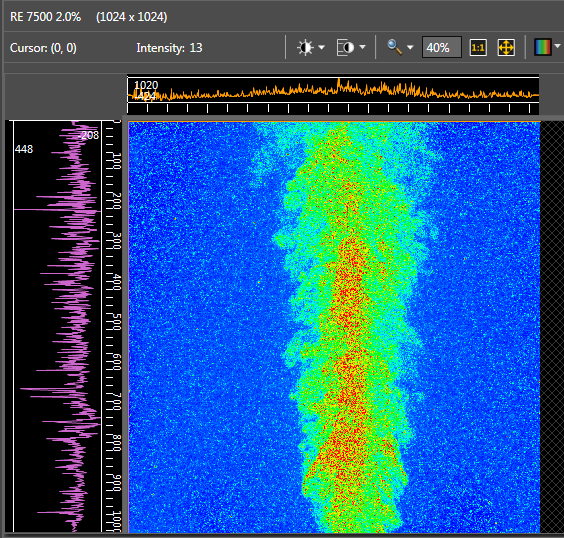
\includegraphics[width=0.55\linewidth]{RE-7500-20-1st.PNG}
    \caption{{\footnotesize Re=7500, 2\% Sample 1}}
\end{figure}
\begin{figure}[h]
    \centering
    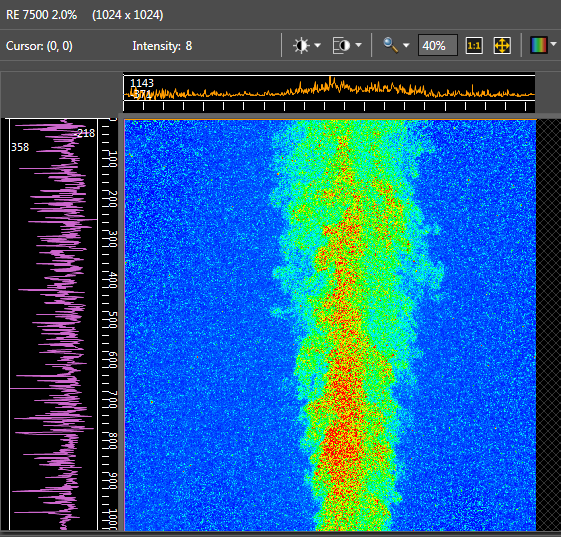
\includegraphics[width=0.55\linewidth]{RE-7500-20-2nd.PNG}
    \caption{{\footnotesize Re=7500, 2\% Sample 2}}
\end{figure}
\begin{figure}[h]
    \centering
    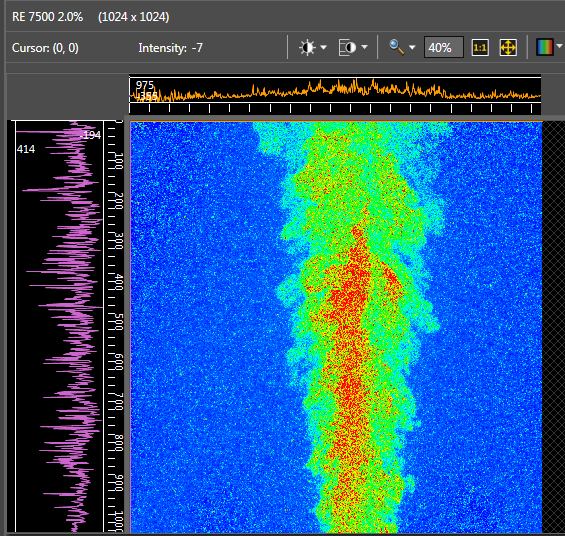
\includegraphics[width=0.55\linewidth]{RE-7500-20-3rd.PNG}
    \caption{{\footnotesize Re=7500, 2\% Sample 3}}
\end{figure}
\begin{figure}[h]
    \centering
    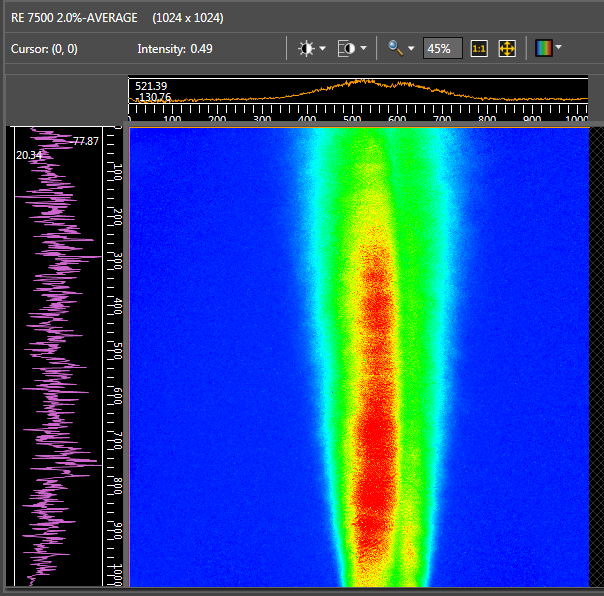
\includegraphics[width=0.55\linewidth]{RE-7500-20-Avg.PNG}
    \caption{{\footnotesize Re=7500, 2\% Average}}
\end{figure}

\begin{figure}[h]
    \centering
    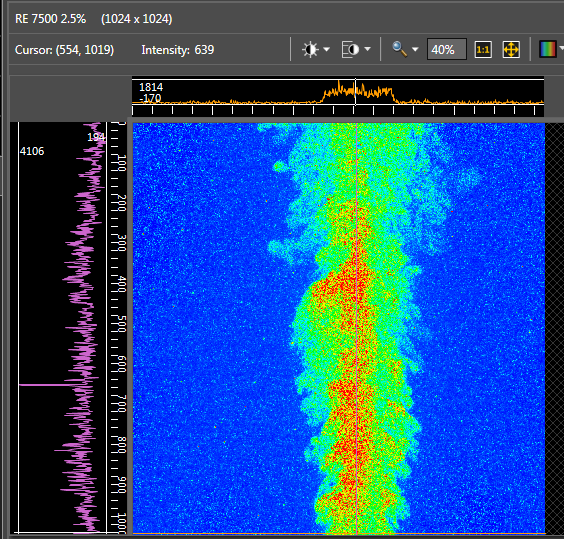
\includegraphics[width=0.55\linewidth]{RE-7500-25-1st.PNG}
    \caption{{\footnotesize Re=7500, 2.5\% Sample 1}}
\end{figure}
\begin{figure}[h]
    \centering
    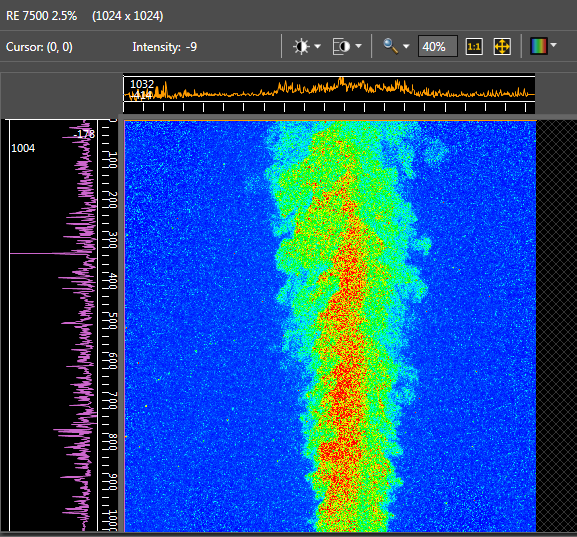
\includegraphics[width=0.55\linewidth]{RE-7500-25-2nd.PNG}
    \caption{{\footnotesize Re=7500, 2.5\% Sample 2}}
\end{figure}
\begin{figure}[h]
    \centering
    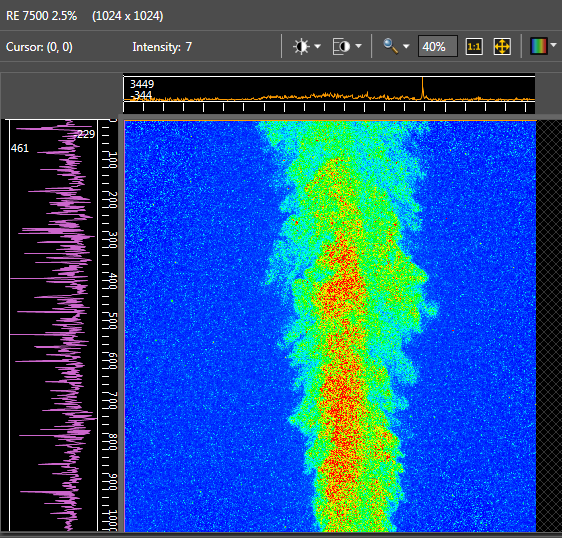
\includegraphics[width=0.55\linewidth]{RE-7500-25-3rd.PNG}
    \caption{{\footnotesize Re=7500, 2.5\% Sample 3}}
\end{figure}
\begin{figure}[h]
    \centering
    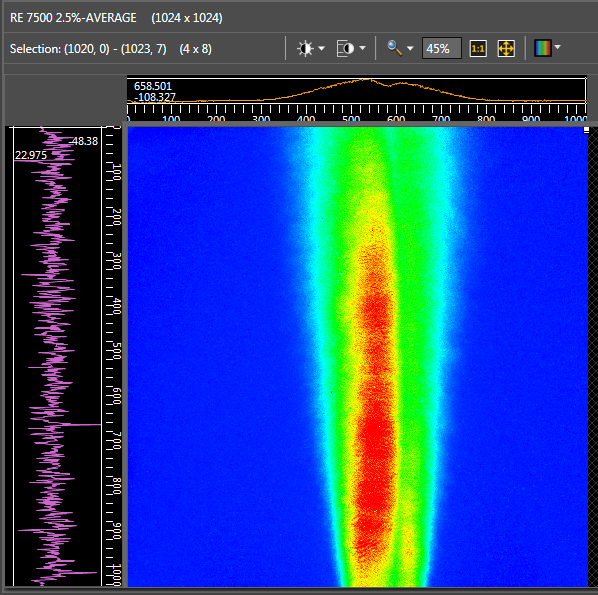
\includegraphics[width=0.55\linewidth]{RE-7500-25-Avg.PNG}
    \caption{{\footnotesize Re=7500, 2.5\% Average}}
\end{figure}




\end{document}